
\documentclass[12pt]{article}
\usepackage[utf8]{inputenc}
\usepackage[a4paper,left=1in,right=1in,top=1in,bottom=1in]{geometry}


%CITATIONS
\usepackage[
backend=biber,
style=authoryear,
giveninits=false,       % No initials in citations
maxcitenames=2,         % Show up to 2 authors in citations before truncating
maxbibnames=999,        % Show all authors in the bibliography
natbib=true,            % For \citet and \citep
dashed=false,           % No repeated names in bibliography
doi=false,
url=false,
eprint=false,
]{biblatex}
\addbibresource{bib.bib}

\DeclareNameFormat{labelname}{%  
	\nameparts{#1}%  
	\usebibmacro{name:family}{\namepartfamily}{\namepartgiven}{\namepartprefix}{\namepartsuffix}%  
	\usebibmacro{name:andothers}%  
}
\usepackage{authblk}

% plottting
\usepackage{graphicx}
\usepackage{float}

%OTHER
\usepackage{pdflscape}
\usepackage{mathrsfs }% for lagrangian
\usepackage{amsmath}
\usepackage{amssymb}
%\usepackage{float}
\usepackage{hyperref} 
\hypersetup{
	colorlinks=true,
	linkcolor=blue,
	filecolor=blue,      
	urlcolor=blue,
	citecolor=blue,
}

%APPEDNDIX
\usepackage{appendix}

%TABLES
%\usepackage{floatrow}
\usepackage{longtable}%table over multiple pages
\usepackage{tabularx}
\usepackage{makecell} % For multi-line cells
\usepackage{array} % For better column formatting
\usepackage{booktabs}
\usepackage{adjustbox}

\title{\vspace{-2.0cm}Driving in the wrong direction? Modelling policy-mixes for electric vehicle adoption\\\textbf{SUPPLEMENTARY MATERIAL}}
\date{}
\author{}


\begin{document}
	\maketitle
	
	\section{Parameter Calibration} \label{Appendix_Callibration}
	This section describes the method chosen to set each of the parameters in the model. Due to the incomplete availability of data, only some of the parameters directly match the real-world data. In order to minimise parameter calibration, we set most of the unobservable parameters at values that are found in previous studies or that lie in a reasonable order of magnitude. For these parameters, we implement the respective sensitivity analyses to fully understand their relevance in the model dynamics. Lastly, the distribution of vehicle users' innovativeness (what proportion of their social network owns an electric vehicle (EV) before they consider purchasing one) is indirectly calibrated using a neural network to match EV uptake in California during 2010 to 2023.   
	
	\subsection{Vehicle choice parameters} \label{Callibration_Consumer}
	
	\textbf{Quality scaling exponent} ($\alpha$): The parameter $\alpha$ serves to create a non-linear relationship between quality and willingness to pay, specifically imposing decreasing returns. Due to a lack of data availability, we set this parameter at $0.5$ and then perform a subsequent sensitivity analysis.
	
	\textbf{Willingness to pay for quality} ($\beta_i$): The parameter $\beta_i$ indicates the subjective willingness to pay an individual $i$ assigns to a given scaled quality value. Given that quality is measured in abstract units, this value is non-observable. However, after determining the other parameters relevant to vehicle choice, the order of magnitude of this parameter is key to determining the price level. For this reason, we indirectly calibrate this parameter to make the optimal price for a car with average features targeted at the most represented segment equal the mean price reported in the literature \citep{Grieco2024MarketPower}, in 2020 prices ($P_{m,s}=\$39,290$).
	
	For this estimation, we assume that the average car is an internal combustion engine vehicle (ICEV), and has average production costs, fuel efficiency, and quality. Furthermore, we assume that the cost and emissions per fuel are the last reported values.
	
	From the optimal price derivation, see section \ref{Appendix_Price_Derivation}, we know that:
	\begin{equation}
		\text{exp}({\kappa U(P_{m,s},\beta_s)}) =  W_s(\kappa(P_{m,s}-C_m) - 1)
	\end{equation}
	Taking the log, we get:
	\begin{equation}
		{\kappa U(P_{m,s},\beta_s)} =  \text{ln}\left(W_s(\kappa(P_{m,s}-C_m) - 1)\right)
	\end{equation}
	Multiplying by $1/\kappa$:
	\begin{equation}
		{U(P_{m,s},\beta_s)} =  \text{ln}\left(W_s(\kappa(P_{m,s}-C_m) - 1)\right) (1/\kappa)
	\end{equation}
	Knowing that from the perspective of the price setter:
	\begin{equation}
		U(P_{m,s},\beta_s)=-P_{m,s}-\gamma_sE_{m}+\beta_sQ_{m}^\alpha+\nu(B_{m}\omega_{m})^{\zeta}-\bar{D}\frac{(1+r)(1-\delta_{m})(c_{m}+\gamma_se_{m})}{\omega_{m}(r-\delta_{m}-r\delta_{m})}
	\end{equation}
	Re-arranging, $\beta_s$ is defined as below:
	\small{
		\begin{equation}
			\beta_s = \frac{1}{Q_{m}^\alpha} \bigg(\text{ln}\left(W_s(\kappa(P_{m,s}-C_m) - 1)\right) (1/\kappa)+P_{m,s}+\gamma_sE_{m}-\nu(B_{m}\omega_{m})^{\zeta}+\bar{D}\frac{(1+r)(1-\delta_{m})(c_{m}+\gamma_se_{m})}{\omega_{m}(r-\delta_{m}-r\delta_{m})}\bigg)
		\end{equation}
	}
	Thus, we obtain the willingness to pay for quality of the median consumer. Following this step, we use the income distribution data from the \href{https://www.bls.gov/cex/tables/geographic/mean/cu-state-ca-income-quintiles-before-taxes-2-year-average-2020.htm}{U.S. Bureau of Labor Statistics} to assign the values of $\beta_i$ to the rest of the individuals in such a way that the same proportion is maintained.
	
	\textbf{Willingness to pay for emission reduction} ($\gamma_i$): This parameter indicates how much a consumer is willing to pay to reduce one kilogram of $CO_2$ per kilometre. We know from \citet{hulshof2020willingness} that on average consumers are willing to pay $\$WTP=\$46646.65434$ (in 2020 dollars) to reduce 1 gram of $CO_2$ per kilometre. The average consumer is indifferent between two cars where the price of the first is the $\$WTP$ more expensive but saves 1 gram of $CO_2$ per kilometre. This is shown in the equality below, where we assume $\gamma_i=\bar{\gamma}$ and $D_i=\bar{D}$
	\begin{align}
		U_{a,i,t}(\gamma_i=\bar{\gamma},D_i=\bar{D},e_{a,t}=e)&=+\$WTP+U_{a,i,t}(\gamma_i=\bar{\gamma},D_i=\bar{D},e_{a,t}=e+\omega_v)\\  
	\end{align}
	Then, we can isolate the willingness to pay, and $\gamma_i$ as follows:
	\begin{align}
		\$WTP &= \frac{\bar{\gamma}\bar{D}(1+r)(1-\delta_{a})}{(r-\delta_{a}-r\delta_{a})}\\
		\bar{\gamma} &= \frac{\$WTP(r-\delta_{a}-r\delta_{a})}{\bar{D}(1+r)(1-\delta_{a})}
	\end{align}
	The willingness to pay for emission reduction $\gamma$ is normally distributed across the population with standard deviation $\sigma=39160.31118$ \citep{hulshof2020willingness}. We assume the distribution of this value is uncorrelated with the other preference parameters, such as willingness to pay for quality or range.
	
	\textbf{Range scaling exponent} ($\zeta$): The parameter $\zeta$ serves to create a non-linear relationship between range and willingness to pay, specifically imposing decreasing returns. \citet{FERGUSON2018208} report that people's willingness to pay per kilometre range is lower for gasoline cars. Potentially, this fact is attributed to the diminishing returns to scale with respect to range \citep{HOEN2014199}. Having the range for both cars ($700$ km ICE, $250$ km EV) and the respective WTP/km ($\$10.09$ ICE, $\$20.83$ EV)\footnote{The survey reports heterogeneity by customer type. We take the weighted average of each WTP to reflect a single representative consumer type}, we proceed to calculate the value of $\zeta$ that solves the system of equations below:
	\begin{align}
		\$10.09 \times 700 = \nu 700^\zeta\\
		\$20.83 \times 250 = \nu 250^\zeta\\
	\end{align}
	Which gives the following solution:
	\begin{align}
		\zeta = \frac{\ln{(\$10.09 \times 700)}-\ln{(\$20.83 \times 250)}}{\ln{(700)}-\ln{(250)}}\\
		\zeta = 0.296
	\end{align}
	
	\textbf{Willingness to pay for range capacity} ($\nu$): This parameter indicates how much a consumer is willing to pay for an extra kilometre in car range. Having calibrated $\zeta$ to match the points in previous empirical studies \citep{FERGUSON2018208}, we solve for $\nu$ in the system below:
	\begin{align}
		\$10.09 \times 700 = \nu 700^{0.2960778787}\\
		\$20.83 \times 250 = \nu 250^{0.2960778787}\\
	\end{align}
	Isolating $\nu$:
	\begin{align}
		\nu=\$10.09 \times 700 / 700^{0.2960778787} = \$1,015.54 \\
		\nu=\$20.83 \times 250 / 250^{0.2960778787} = \$1,015.54\\
	\end{align}
	Since this study uses 2015 data, we translate it to 
    2020 prices using the California CPI \href{https://dof.ca.gov/forecasting/economics/economic-indicators/inflation/}{State of California Department of Finance}, giving us a value of $\$1,173.65$.
	
	\textbf{Distance travelled} ($D_i$): This parameter scales a consumer's willingness to pay for savings in fuel costs and fuel emissions. We assign the parameter values to the different drivers in our model based on surveys using self-reported data about their yearly mileage from the \href{https://www.energy.ca.gov/data-reports/surveys/california-vehicle-survey/vehicle-miles-traveled-fuel-type}{California Energy Commission}. We simplify in the following fashion: First, we assume that distance is equally distributed over the year. Second, we only take the distribution of distances travelled for new cars, even though they slightly decrease as cars get older. Third, given that the survey data is distributed in ranges, we assign the mid-point to each consumer belonging to a bin. Fourth, given that the last range includes people who drive more than $25,000$ miles per year, we assume that the range midpoint is $1.5$ times that value. Finally, we assume the distribution of monthly mileage is uncorrelated to other preference characteristics. 
	
	\textbf{Discount rate} ($r$): This parameter influences the relevance of making savings in the future from considering cars with greater efficiency, or EVs when the price and emissions of electricity are lower than those of gasoline. We use a value of $5\%$ yearly discount rate, which gives a monthly value of $0.407\%$. This rate is common in other emprical and modelling literature related to car purchases \citep{woody2024electric, busse2013consumers, greene2010consumers}, with is value corresponding to near average values of car loan APRs.
	
	\textbf{Consumer intensity of choice} ($\kappa$): This parameter determines the degree of rationality in consumer choice, ultimately affecting the speed of EV uptake when EVs become superior to ICE cars. Furthermore, it affects prices as firms optimally levy higher mark-ups when consumers feature bounded rationality. Given that the logit choice model weights the absolute consumer surplus, the value of $\kappa$ alone is not informative about the degree of rationality consumers feature. It is set through a grid search that balances prices, market concentration and firm markups to match those found in \citet{Grieco2024MarketPower}.
	
	\subsection{Social network parameters} \label{Callibration_SocialNetwork}
	
	\textbf{Network density and re-wiring}: To represent the medium over which vehicle users interact a Stogatz-Watts small-world network \citep{watts1998collective} is employed. In this network, neighbours are highly clustered triads whereby two neighbours of an individual are likely to be neighbours. The network is generated by first forming a ring of vehicle users each connected to their nearest neighbours, such that node degree is homogenous, then with a given probability $p_{WS}$ one end of link between vehicle users is moved to another random user. This re-wiring produced the small world property whereby the network has a short path length due to a few cross-network connections. To test different network sizes, a network density is set $\rho_{WS}$, instead of setting a fixed number of connections per vehicle user. Thus the mean number of connections per vehicle user is given by $N_{SW} = (I- 1)\rho_{WS}$. The network density is 
	a key in determining how sparse connections are, making it more likely to have clusters of non-adopters whenever density is low. Due to a lack of data availability, we fix this parameter at $\rho_{WS} = 0.05$ and perform a subsequent sensitivity analysis. 
	
	\textbf{Degree of innovativeness} ($\chi: \alpha_{\chi},\beta_{\chi}$): This parameter determines the threshold of EV adopters in someone's network before the individual considers buying an EV. It is crucial to determine the speed of EV uptake once EVs begin to outperform ICEVs. We represent the distribution of $\chi$ values using a beta distribution. Due to its relevance and lack of data availability, the two parameters that characterise the innovativeness distribution $\alpha_{\chi},\beta_{\chi} $ using simulation-based inference \citep{papamakarios2016fast,cranmer2020frontier, dyer2024black} to match EV uptake during the validation period. Specifically, we use the neural poster estimation method from the \textit{sbi} python package \citep{tejero-cantero2020sbi}. In this method, the outputs of the ABM are used to train a mixture density network that estimates a posterior for the values of $\alpha_{\chi},\beta_{\chi}$. Each simulation run for a given parameter setup, generates the output vector of yearly EV uptake, in October, during the validation period, these are compared to the real-world uptake data. After an initial round of simulation the posterior estimation generated by the mixture density network can generate new prior values of $\alpha_{\chi},\beta_{\chi}$, narrowing down the range to be explored in the next round. Thereby generating more accurate predictions in a computationally efficient manner. Once training rounds are completed, the posterior is sampled to indicate what values $\alpha_{\chi},\beta_{\chi}$ give the best fit, \ref{fig:inference}. The best suggested values are tested, with a priority given to those that better match more recent EV adoption data.
	
	\subsection{Exogenous car parameters} \label{Callibration_CarParams}
	
	\textbf{Gasoline and electricity cost per kilowatt hour} ($c_{v,t}$): These exogenous variables are type-specific and influence the relative attractiveness of EVs, both in relative terms and in absolute terms, given that EVs have higher fuel efficiency. For ICE cars, we take the monthly cost per gallon in California reported by the EIA (\href{https://www.eia.gov/petroleum/gasdiesel/}{EIA}) and use the kWh equivalent per gasoline gallon (\href{https://afdc.energy.gov/fuels/properties}{AFDC}). For EVs, we use the monthly price of residential electricity per kWh in California (\href{https://www.eia.gov/opendata/browser/electricity/retail-sales}{EIA}). For months with incomplete data, we assume the value equals that of the closest month with reported values. Figure \ref{fig:Costs_Electricity_Gasoline} shows the evolution of both variables.
	
	\textbf{Gasoline and electricity emissions per kilowatt hour} ($e_{v,t}$): These exogenous variables are type-specific and influence the relative attractiveness of EVs, both in relative terms and in absolute terms, given that EVs have higher fuel efficiency. For ICE cars, we take the assumed value in the 2022 IPCC Mitigation report \citep[Table 10.8]{ipcc2022transport} and transform it to kg of $CO_2$ per kWh. For EVs, we use the monthly data for average emissions intensity in the Californian electricity grid (\href{https://ember-energy.org/data/us-electricity-data-explorer/}{EMBER}). For months with incomplete data, we assume the value equals that of the closest month with reported values. Figure \ref{fig:Emissions_Electricity_Gasoline} shows the evolution of both variables.
	
	\textbf{ICE car and EV manufacturing emissions} ($E_{v,t}$): These parameters influence the willingness to pay for new cars of environmentally-concerned consumers. We use the production emissions estimated by the IPCC 2022 mitigation report \citep[1076]{ipcc2022transport}, where the manufacturing emissions of EVs are estimated at $14$ tonnes of $CO_2$ and those of ICE cars are estimated at $10$ tonnes of $CO_2$.
	
	\textbf{ICE car and EV fuel efficiency depreciation rate} ($\delta$): These parameters influence the speed at which consumers change their car and diminish the long-term advantages of cars with higher fuel efficiency. Under the constraint that $\delta<\frac{r}{1+r}$, we know the value is upper bounded at $0.246\%$. Given that, we fix the monthly depreciation rate for both car types at $0.18\%$ and perform a subsequent sensitivity analysis. This value is set so that the average age of vehicles matches that of our stylized facts (10-12 years old), see \href{https://www.bts.gov/content/average-age-automobiles-and-trucks-operation-united-states}{Bureau of Transportation Statistics}.
	
	\textbf{Scrap value} ($F$): The scrap value increases the speed at which consumers change their car as it increases the minimum price paid by the used car merchant, and therefore decreases the net cost from buying a new or used car. We assume a scrap value of $\$669.80$, which is the reported value in a specialised source \href{https://junkcarsus.com/prices}{JunkCarsUS}.
	
	\textbf{Price depreciation rate for used cars} ($\xi_{v,t}$): The price depreciation rate for used EVs and ICE cars has an ambiguous effect. On the one hand, it increases the probability that a used car is bought as it reduces its selling price. On the other hand, it reduces the number of periods before it gets disposed. Its effect on the overall sale of used cars depends on its interaction with the fuel efficiency depreciation rate and the scrap value. We set these parameters based on previous studies \citep{SCHLOTER20222Depreciation}, we set a monthly depreciation rate of $.87\%$ for ICE cars and one of $1.16\%$ for EVs.
	
	\textbf{Used car dealer mark-up} ($\mu$): This parameter affects the speed at which price-sensitive vehicle users change their car, given that larger values of $\mu$ decrease the revenues from selling a user's own car. Lacking reliable information on the actual target mark-up for used cars, which is heterogeneous across used car dealers, we fix this parameter at $100\%$ and perform the subsequent sensitivity analysis afterwards.
	
	\subsection{NK landscape parameters} \label{Callibration_NK}
	
	\textbf{Number of components} ($N$): The number of components affect the performance distribution across technologies. Given that the performance of an attribute equals the average of $N$ draws from a uniform distribution, the distribution of performances over the $2^N$ existing technologies approaches the normal distribution as $N$ grows larger. For this reason, we fix $N=15$ as a number sufficiently large to ensure that property. We assume the NK landscapes for ICE cars and EVs are equally large.
	
	\textbf{Landscape complexity} ($K$): The degree of complexity increases the number of local solutions in the search process, hence decreasing the probability a local-searching agent finds a global solution. As $K$ approaches $N-1$, the search process becomes closer to a random draw from a normal distribution. Since the purpose of incorporating NK landscapes into this model is to integrate the role of structured search in determining path-dependent industrial transformation in the context of multiple attributes, we select an intermediate level of complexity that ensures the existence of "local traps" while maintaining past search relevance. We fix $K=3$ and perform the subsequent sensitivity analysis afterwards. We assume the NK landscapes for ICE cars and EVs are equally complex.
	
	\textbf{Attribute performance correlations} ($\rho$): This vector of parameters determines how correlated are the performance of the difference attributes, potentially creating trade-offs when choosing research paths. To account for the main cost driver in EV manufacturing \cite{konig2021overview}, we include an additional component of innovation for EVs, the battery size. This means that firms cannot easily produce EVs with high battery capacity for a low-cost consumer market due to additional innovation complexity. We assume that the correlation of production costs with quality, fuel efficiency, and battery size are zero. In doing so, despite of setting the boundaries of each attribute as the currently existing best technology, the model allows for radical innovations by enabling technologies that render the existence of high-quality and efficiency cars at a low cost.  
	
	\textbf{Quality upper and lower bounds in the NK landscape} ($Q^-,Q^+$): Quality is a catch-all variable for all other relevant features that determine the price of a car, such as comfort, style, horsepower, or other appliances \citep{ostli2017generic,Grieco2024MarketPower}. Since this combined measure cannot be observed in real-world data, we create an abstract score that scales in the range $(0,1)$. Furthermore, we assume that these boundaries are identical in the ICE and EV landscapes, as the main differences, such as battery autonomy, fuel tank and fuel efficiency, are already included in our analysis.
	
	\textbf{Production costs upper and lower bounds in the NK landscape} ($C^-,C^+$): 
	In setting production boundaries, we represent possible values across a very broad timeline: during the burn-in period, calibration period, policy period and long-term trends. Therefore, we cannot find adequate data sources as our NK landscape does not allow for radical innovation that changes these boundaries. Instead, we take reference order of magnitude values for production costs, sales price, and car markups from literature \citep{konig2021overview, woody2024electric, Grieco2024MarketPower} and then perform grid search until the vehicle prices match those found in our stylized facts during our calibration period.
	
	\textbf{Fuel tank and battery capacity bounds in the NK landscape} ($B^-,B^+$): We assume that fuel tank size has reached technological maturity and all cars have the same value. Therefore, we fixed it at $469.4$ kWh, after converting the fuel tank size of the four most sold cars in California in 2020, see\href{https://www.cncda.org/wp-content/uploads/Cal-Covering-4Q-20.pdf}{California Auto Outlook}, and their associated fuel efficiency, then converting gallons of gasoline to kWh. The battery capacity for EVs is heterogeneous and can benefit from innovation. Based on \citep{Schmuch2018}, we set the maximum value for battery capacity and apply the adjustment described in section \ref{Appendix_NKProperties} to obtain the values for the NK landscape boundaries. Fixing the lower bound at $0$, we reach an upper bound of $150$ kWh.
	
	\textbf{Fuel efficiency bounds in the NK landscape} ($\omega^-,\omega^+$): We take the values from the IPCC 2022 Mitigation report \citep[Appendix 10.2]{ipcc2022transport} and use the adjustments described in section \ref{Appendix_NKProperties} to obtain the values for the NK landscape boundaries. The observed fuel efficiency values for gasoline vehicles range from $1.25$ to $2.62$ km/KWh \footnote{We converted the units of the IPCC report using a factor of 0.278 KWh per MJ}, leading to lower and upper bounds in the NK landscape of $.791$ and $3.087$. For EVs, the IPCC reports values efficiency ranges of $4.132$ to $8.333$, leading to lower and upper bounds in the NK landscape of $2.731$ and $9.734$. 
    
    To compare our calibration with real-world cars in Figure \ref{fig:calibration_cars} we plot car range and cost for simulated ICEV and EVs for 64 seed runs and a total of 3142 total cars. Additionally, we include data on a representative sample of common cars available in 2025 from \href{fueleconomy.gov}{www.fueleconomy.gov}\footnote{Accessed on the 30th of April 2026}. The simulated cars are all cars on sale in December 2023, at the end of the calibration period. In the the case of EVs, the target type of car for the policy period, we match data well on both price and driving range. It is important to note that neither of these variables is directly calibrated in the model, and are emergent properties of the simulation. In the case of ICEVs, the calibration is on price is reasonable but high, whilst the driving range is approximately 20\% too large. We attribute this discrepancy to our calibration choice of fixing the fuel tank size to the top tier found in real-world data (see Section 1.3 of the Supplementary Material).
	
	\subsection{Car manufacturer parameters} \label{Callibration_Manufacturer}
	
	\textbf{Segment partitions} ($R$): The number of segment partitions on each segment influences the degree of heterogeneity in products in the market and emphasises the path-dependent nature of firm specialisation. Together with the parameters that influence the path-dependence of search ($K,\lambda$), this vector of parameters ultimately affects market concentration. We fix the number of partitions at $8$ in the $\beta$ (quality/luxury) space and $2$ in the $\gamma$ (environment) space. For robustness, we perform the subsequent sensitivity analyses. The high segmentation in quality space allows for more diversity in car models, reflecting low concentration in real-world markets.
	
	\textbf{Research intensity of choice} ($\lambda$): This parameter balances exploitation and exploration during the search process. For high values of landscape complexity ($K$), a low value of ($\lambda$), relative to the order of magnitude of expected profits, helps firms escaping local solutions. We set this value at $1e-3$ and perform the subsequent sensitivity analyses. 
	
	\textbf{Firm memory size} ($M^+$): As in the research intensity of choice ($\lambda$), there is a trade-off in setting the firm memory size. A large memory size contributes to research exploitation by avoiding the repetition of research efforts. However, if an agent has all neighbouring technologies in memory it remains permanently stuck until one of them is forgotten. We set the memory size at the exact amount to make possible, yet highly unlikely, a permanent stuck position $M^+=30$, given that each of the two landscapes has $15$ neighbouring points in every position. 
	
	\subsection{Event-based probabilities} \label{Callibration_Events} 
	
	The probability that a vehicle users considers changing its car ($\eta$), a car manufacturer consider changing its supply line and prices ($\theta$), and the probability a car manufacturer succeeds at innovating ($\iota$) are set in such way that, on average, these events occur once per year ($1/12$). The greater this probabilities the faster that co-evolutionary processes can occur as consumer adapt faster to changing product offerings and firms adapt faster to consumer desires. The higher the probability the greater the computational cost of the simulation. This applies especially for $\eta$ as utility calculations for a greater proportion of the population carry significant computational load.
	
	\section{Sensitivity Analysis} \label{Calibration_Sensitivity}
	\subsection{Local sensitivity analysis}
	Figure \ref{fig:sensitivity} shows the sensitivity of key model parameters in the simulated EV uptake projections for the period 2001-2023. We test the sensitivity of the quality scaling component (panel A), the discount rate (panel B), the used car dealer mark-up (panel C), the consumer intensity of choice (panel D), the parameters governing the chi distribution of the imitation threshold (panels E and F), the research intensity of choice (panel G), the fuel efficiency depreciation rate (panel H), and the technology complexity in the EV and ICEV landscapes (panels I and J). 
	
	The quality scaling component negatively impacts EV adoption as it increases the relevance of attributes that are superior among existing ICEVs due to research advantage developed during the burn-in period. The discount rate negatively impacts EV adoption as it diminishes the utility contribution of the long-run benefits of adopting an EV. These benefits are the monetary and emissions savings derived from better fuel efficiency. The mark-up in the market for used cars has a small positive effect on EV adoption as it makes the long-term aspects of car evaluation relatively more important than its short-term counterparts.
	
	The consumer intensity of choice has a positive effect on EV adoption as consumers become more likely to adopt EVs when they become a superior alternative to ICE cars. EV uptake increases when the distribution of the imitation threshold is left-skewed, favouring social diffusion. A left-skewed distribution corresponds to high values of $b_\chi$ and low values of $a_\chi$.
	
	In the case of the research intensity of choice, we find that EV uptake increases when research choices become more random. This is caused by the fact that the policy incentives favouring EV penetration become more relevant than the initial advantage that ICEVs gain over EVs during the burn-in period via research. Additionally, when the pool of potential EV users is small a more stochastic approach to research leads to more EV designs chosen, despite of lower expected profit. The fuel efficiency depreciation rate negatively affects EV uptake because fuel efficiency is the main advantage that EVs have over ICEVs.
	
	The EV landscape complexity has a negligible effect on EV uptake, due to a small numbers of EV sold during the calibration period. Conversely, the ICE landscape complexity has a mixed but significant effect on the EV uptake. On the one hand, with high complexity the likelihood of finding good innovations decreases due to a higher number of local solutions. This makes innovation in the EV landscape more effective. On the other hand, EV uptake increases when the complexity in the ICEV landscape is low as it reduces the variety of technologies that are developed. Lastly, when stochastic seeds are varied to give a confidence interval we assume that the inputs to the model are fixed, thus we only test changes in the dynamics of the model. However, by varying the complexity of the landscape, we change the inputs. This means that differences between complexity runs may also be due to different seeds in the landscape generation.

    \subsection{Global Sensitivity}
	To complement these local sensitivity analyses, we additionally perform a Sobol sensitivity analysis \citep{sobol2001global}, using the SALib Python library \citep{Herman2017}, see Figure \ref{fig:sobol_first} and Figure \ref{fig:sobol_total}. 
	
	The simplest outputs to explain are those of EV adoption proportion, market concentration, utility and mean car age. These have one or two key parameters and high first-order Sobol values, indicating limited interaction between parameters. 
	
	In the case of EV adoption, it is dominated by the $a_{\chi}$ that forms one-half of defining the beta distribution of innovativeness thresholds in the model. Specifically, a larger value of $a_{\chi}$ results in a greater threshold and, thus, more social lock-in to prevent EV adoption. We also note the small role that the discount rate $r$ has in EV adoption due to greater values of this parameter, which makes the long-term benefits of EVs less attractive and thus lowers EV adoption likelihood. 
	
	The beta distribution parameter $a_{\chi}$ also dominates the market concentration. HHI remains relatively stable with no EV transition due to the long burn-in period; however, if an EV transition occurs, HHI increases rapidly, resulting in greater variance over different $a_{\chi}$ that determines EV adoption rates. 
	
	In the case of utility, the quality diminishing returns factor, $\alpha$, generates more utility for the same car if it has a higher value. However, of greater influence is the consumer intensity of choice, $\kappa$, the greater its value, the more individuals maximise utility, but additionally, the lower firm profits mean a corresponding drop in vehicle prices.
	
	In the case of the mean car age, the key parameter is the car efficiency decay $\delta$; the greater its value, the faster the vehicle fleet has to be replaced, thereby lowering the car age. Additionally, if an EV transition occurs, then vehicle users purchase cars ahead of schedule, due to the efficiency and lower running costs of EVs, thereby lowering the car age of the fleet, hence the importance of $a_\chi$. 
	
	In the case of cumulative emissions and firm profit, we see a divergence between the importance of parameters between the Sobol first and total order indices. Both outputs are correlated in part because the sale of a vehicle results in large production emissions and firm profits.
	
	In the case of cumulative emissions parameters, determining EV adoption plays a key role, but additionally, those such as the used car deal markup are also of importance. In the case of this markup, the greater the value, the lower the trade-in value of used cars is, thus the lower the incentives for individuals to change their cars, resulting in less frequent purchasing of vehicles (either new or used). This change in purchase frequency may have an indirect effect on the production emissions as those purchasing used cars may do so more often, whilst the purchase frequency of new cars remains fixed (due to lower relative price sensitivity). This would also account for the lack of influence of $\mu$ on the mean car age, and the effect of $\mu$. In the case of the Epistasis parameter for ICEVs, $K_{ICE}$, greater landscape complexity may result in lower production emissions as consumers do not see significant technological advances between vehicle purchasing opportunities. 
	
	In the case of firm profits, the consumer intensity of choice $\kappa$ is a key parameter due to greater values driving down prices. Second, greater values of the fuel efficiency decay rate $\delta$ result in more frequent purchasing behaviour of new cars as the utility of used hand cars decay more quickly.  

    \subsection{Policy Sensitivity}
    We complement our sensitivity analysis with a grid search evaluating how the minimum policy intensity required to achieve the EV uptake target in 2035 reacts to changes in key parameters of our model. For this analysis, we select the only two policies that achieve such target (carbon prices and new car rebate) and the two most sensitive parameters: the willingness to pay for quality $\beta$ and the distribution of the innovativeness parameter $\chi$.
    
    The inverse of the willingness to pay for quality ($1/\beta$) is a proxy for the price sensitivity of consumers, given that it reduces the weight of quality in a car's evaluation, thus making the lifecycle costs (and the policies affecting it) more relevant. Since this parameter is heterogeneous across the population of car users, we adjust it with a scale multiplier.

    In Figure \ref{fig:WTP_sensitivity_carbon_price} and Figure \ref{fig:WTP_sensitivity_adoption_subsidy} we observe that the effect of the carbon price and the new car rebate on 2035 EV uptake reacts positively to reductions in $\beta$. As a result, the required policy intensity to meet the same target is lower. The required carbon price is more than halved when all $\beta_i$ are divided by four. This is because a lower value leads to a population that is more price-sensitive as quality represents a smaller proportion of a car's utility. This results in higher EV uptake due to the lower lifecycle costs of EVs given their higher efficiencies.

    The parameter $a_{\chi}$ controls the skew of the distribution of individual innovativeness thresholds $\chi_i$. This parameter determines the threshold of EV adopters in someone’s network before the individual considers buying an EV.  A lower value of $a_{\chi}$ means more of the population is innovative and willing to consider purchasing an EV if a smaller proportion of their neighbours owns one. 
    
    Figure \ref{fig:a_chi_carbon_price} tests a range of carbon prices and $a_{\chi}$ values. By lowering its value, we can generate higher EV uptake for a lower policy intensity of carbon price, but then this moves the BAU scenario out of the calibrated range. The non-linearity exhibited in Figure \ref{fig:a_chi_carbon_price} demonstrates the strength of our threshold model in generating social lock-in phenomena. More precisely, for a sufficiently large $a_{\chi}$ (i.e. a laggard society), even extreme policy values do not cause a proportional increase in EV uptake. Conversely, for a sufficiently small $a_{\chi}$ (i.e. an innovator society), large EV adoption is realised even in the BAU scenario, rendering the policy superfluous.

    \subsection{BAU sensitivity}
    \label{bau_sensitivity}

    In Figure \ref{fig:BAU_sen_elec}, we test the relevance of grid decarbonisation and electricity prices in our results. The simulations span over the extended policy period (2024-2050) covering nine scenarios comprising the combinations of three electricity price changes (50\% decrease, no change, and 50\% increase) and three grid decarbonisation scenarios (90\%, 50\% and 25\%). We observe that electricity prices have a sizeable effect on EV uptake, as suggested by our policy analysis results, highlighting the effectiveness of electricity subsidies. On the other hand, reducing the emissions intensity of the power grid has little effect on EV uptake, given that financial incentives dominate environmental preferences for most consumers. Furthermore, the high efficiency of EVs mitigates the marginal effect of emissions per kWh on driving emissions. However, in the case of high EV uptake, grid decarbonisation is relevant for the flow of emissions. The effect of prices on emissions is stronger than grid decarbonisation itself, as for the electricity grid to play a role in reducing emissions, there must already be a large number of EVs on the road. This emphasises the relevance of tandem transitions to achieve stronger decarbonisation.

    In Figure \ref{fig:BAU_sen_elec_elas}, we test the relevance of grid decarbonisation and electricity prices in our results. The simulations span over the extended policy period (2024-2050). The Figure evaluates the effect of a 1\% increment in electricity prices on EV uptake (top right) and cumulative emissions (bottom right) for a 50\% increment (dark blue) or reduction (light blue) from its last reported value. Likewise, it evaluates the effect of 1\% increment in grid decarbonisation on EV uptake (top left) and cumulative emissions (bottom left) for a 50\% reduction (dark red) or 90\% reduction (light red) from its last reported value.
    
    The first observation is that the marginal effect of either parameter on EV uptake diminishes with scale. This can be deduced from the fact that the elasticity is higher for low values of electricity price (top right) or grid intensity (top left). On the other hand, the elasticity of either parameter on cumulative emissions is constant with respect to the scale. This is attributed to the non-linearities of the social imitation model influencing EV adoption. 
    
    Second, the effect of electricity prices outweighs that of grid intensity by a factor of 10 on EV uptake and by a factor of 3. The fact that prices have a stronger influence on EV uptake, due to the higher relevance of financial over environmental aspects, results in a greater impact on emissions too. 
        
	\section{The technology landscape} 
	\subsection{How NK landscapes work} \label{Appendix_NK}
	The development of car types is the result of combining different inputs such as frame components, engines, transmission components, batteries, interior and exterior components. From each component, the car producer has a variety of types, shapes or materials to choose from. The choice of which input type to use for the manufacturing of a car has direct and indirect effects on the overall attributes of the final good, provided that the components of a vehicle often complement each other.
	
	We employ $NK$ models \citep{kauffman1993origins, levinthal1997adaptation} to capture the complexity inherent in product design choices. An $NK$ landscape maps all possible input combinations to a fitness outcome. In a stylized and deterministic manner, the modeller can adjust the extent to which the fitness of a specific input combination can be inferred from a sufficiently large record of alternative fitness combinations. This is achieved by modifying the interdependence among inputs, represented by the parameter $K$. This parameter defines the number of inputs whose states influence the performance contribution of a given input. In other words, $K$ serves as a proxy for the underlying complexity of the problem represented in the $NK$ model.
	
	In our model, the fitness values in the $NK$ landscape represent features of the vehicle that ultimately determine the manufacturer’s profits for a given input combination. These features include production costs, vehicle quality, and fuel efficiency. As in prior applications of $NK$ models \citep{adner2014positioning, csaszar2016mental}, we represent fitness as a vector of attributes. This approach is justified by evidence \citep{horne2005improving, ostli2017generic} that consumers consider multiple factors when selecting a vehicle.
	
	An $NK$ landscape is a discrete hypercube where each vertex represents a combination of inputs in specific states. Let $N$ be the set of components. Each component, indexed by $n \in {0, \ldots, N-1}$, assumes a discrete state $\phi_n$ from $\Phi \in \mathbb{Z}$ possible states. As is standard in $NK$ models, we reduce the number of states to a binary choice. Each unique combination of input states ($\Vec{\phi}_{n,m}$) corresponds to a specific variant $m \in M$. The index $m$ is derived by converting the binary string of input states to a decimal representation. 
	
	The $NK$ model assigns a vector of feature values to each combination of input states. In its generalized form, these feature values are denoted as $\vec{o}_{f,m}$. Each component of this vector corresponds to a normalized fitness value $o_{f,m} \in (0, 1)$ for a specific attribute $f$. Following \citep{adner2014positioning}, we generate correlated distributions of feature values, with the parameter $\rho_{f} \in [-1, 1]$ controlling the correlation of each feature $f$ relative to a baseline feature $f=0$. The fitness distribution for $f=0$ is defined first with $\rho_{0} = 1$ by construction.
	
	For each component $n$, we define a subset $N_{n} \subset N$ that includes component $n$ and $K$ additional components. This subset determines the inputs whose state combinations influence the performance contribution of $n$ across all features. Interdependent components are typically selected sequentially, but alternative structures, such as randomized or clustered interdependence, can be adopted depending on the application. 
	
	We construct a "performance matrix" with $|N|$ columns and $2^{K+1}$ rows. Each cell in this matrix is assigned an independent random draw from a distribution $\mathbb{D} \in (0, 1)$. This value represents the normalized performance contribution of a component $n$ to the baseline feature $f=0$, conditional on the specific input state combination in $N{n}$.
	
	To generate fitness contributions for other features ($f \neq 0$), we assign each feature a subset $N_{f} \subset N$ of $\lfloor \rho_{f} |N| \rfloor$ components. For components in this subset, the fitness contribution for the characteristic $f$ matches that for $f=0$ if $\rho_{f} > 0$ and is equal to $1 -o_{0,n,m}$ if $\rho_{f} < 0$. For components not in $N_{f}$, the contribution is independently drawn from $\mathbb{D}$. The performance matrix thus contains a vector of fitness contributions for each input combination across all features.
	
	To compute the total fitness vector for a technology $m \in M$, we average the performance contributions of its components for each feature. This is achieved using the row in the performance matrix corresponding to the binary to decimal transformation of the input state combinations in $N_{n}$. Finally, the absolute performance values for each feature $f \in F$ are normalized by Min-Max scaling, as shown in Equation \ref{EQ_NKFeature}:
	
	\begin{equation} 
		o_{f,m} =o^-_{f} + \left(o^+_{f} -o^-_{f}\right) \frac{1}{|N|} \sum_{n=0}^{N_z}o_{n,f,m}
		\label{EQ_NKFeature} 
	\end{equation}
	
	Where $Y^-_{f}$ and $Y^+_{f}$ are the lower and upper bounds of feature $f$.
	
	\subsection{NK landscape properties} \label{Appendix_NKProperties}
	The $NK$ landscape generates a range of values rather than a specific value in itself. We can set the upper and lower bounds of each attribute's performance contributions. However, given that the actual performance is the average of $N$ iid draws, the actual performance is not likely to be the input parameter. Figure [X] shows some properties of $NK$ landscapes for $N=15$ (a large $N$ is required to generate normally distributed values). We find that the normalized performance values are in the range $(.2,.8)$ with mean and median of $0.5$.\\
	
	We want to find the boundaries ($F^-,F^+$) in the $NK$ landscape that give us $Q^-,Q^+$, knowing that:
	\begin{equation}
		\begin{aligned}
			Q^- = F^- + 0.2(F^+-F^-)\\
			Q^+ = F^- + 0.8(F^+-F^-)
		\end{aligned}
	\end{equation}
	Subtracting both sides we get:
	\begin{equation}
		Q^+-Q^- = 0.6(F^+-F^-)
	\end{equation}
	Then we can isolate:
	\begin{equation}
		F^+-F^- = (Q^+-Q^-)/0.6
	\end{equation}
	Substituting in both equations we get:
	\begin{equation}
		\begin{aligned}
			Q^- = F^- + 1/3(Q^+-Q^-)\\
			Q^+ = F^- + 4/3(Q^+-Q^-)
		\end{aligned}
	\end{equation}
	Isolating $F^-$ we get:
	\begin{equation}
		F^- = (4/3)Q^--(1/3)Q^+ 
	\end{equation}
	Substituting $F^-$ we can isolate $F^+$ as:
	\begin{equation}
		F^+ = Q^+(4/3)-Q^-(1/3)
	\end{equation}
	As a general expression, where $\pi^+,\pi^-$ are the respective percentages we are targeting:
	\begin{equation}
		\begin{aligned}
			F^-=\frac{Q^-\pi^+-Q^+\pi^-}{\pi^+-\pi^-}\\
			F^+=\frac{Q^+(1-\pi^-)-Q^-(1-\pi^+)}{\pi^+-\pi^-}
		\end{aligned}
	\end{equation}
	
	\section{Lifecycle evaluation derivation}\label{Appendix_Lifecycle_Derivation} 
	For an infinite geometric series $\sum_{t=0}^\infty Yx^t$, where $|x| < 1$, the sum is $\frac{Y}{1-x}$. With no loss of generality, we ignore the case where the user is evaluating its own car. We make the following notation simplifications:
	\begin{align}
		C = E_{a} \vee P_{a,t}-\hat{P}_{i,t}\\
		z = c_{a,t} \vee e_{a,t}
	\end{align}
	\begin{align}
		LCC_{a,i,t} &= C + \sum_{t}^\infty D_i \frac{z}{\omega_{a,t}(1+r)^t(1-\delta_{a,t})^t}\\
		&=C + \frac{D_iz}{\omega_{a,t}}\sum_{t}^\infty  \left(\frac{1}{(1+r)(1-\delta_{a,t})}\right)^t\\
		&=C + \frac{\frac{D_iz}{\omega_{a,t}}}{1-\frac{1}{(1+r)(1-\delta_{a,t})}}\\
		&=C + \frac{\frac{D_iz}{\omega_{a,t}}}{\frac{(1+r)(1-\delta_{a,t})-1}{(1+r)(1-\delta_{a,t})}}\\
		&=C + \frac{\frac{D_iz}{\omega_{a,t}}}{\frac{(1+r)(1-\delta_{a,t})-1}{(1+r)(1-\delta_{a,t})}}\\
		&=C + \frac{\frac{D_iz}{\omega_{a,t}}}{\frac{1+r-\delta_{a,t}-r\delta_{a,t}-1}{(1+r)(1-\delta_{a,t})}}\\
		&=C + \frac{(1+r)(1-\delta_{a,t})D_iz}{\omega_{a,t}(r-\delta_{a,t}-r\delta_{a,t})}\\
	\end{align}
	This converges if $|\frac{1}{(1+r)(1-\delta)}|<1$, for which we require $r>\frac{\delta}{1-\delta}$.
	
	\section{Optimal Price Derivation} \label{Appendix_Price_Derivation}
	The price for a car $m$ is set to maximise expected profit in a given segment $s$:
	\begin{equation}
		\mathbb{E}(\Pi_{m,s,t}(P))=\frac{(P-C_{m,t})|I_{s,t}|\text{exp}\left(\kappa U_{m,s,t}(P)\right)}{\text{exp}\left(\kappa U_{m,s,t}(P)\right)+\sum_{m=0}^{Y_{t-1}}\text{exp}\left(\kappa U_{m,s,t}(P)\right)} 
	\end{equation}
	The optimal price satisfies profit maximization:
	\begin{equation}
		P^*_{m,s,t}=\text{argmax}_P \mathbb{E}\left(\Pi_{m,s,t}(P)\right)
	\end{equation}
	The price setter assumes the distance travelled equals the average distance of the entire population ($D_s=\sum_i^{I}{D_i}/|I|$) and disregards the price at which consumers can sell their car ($\hat{P}_{s,t}=0$). In what follows we use the simplifying notation below:
	\begin{equation}
		\begin{aligned}
			O_{m,s,t}= -\gamma_iE_{a}+\beta_iQ_{a,t}^\alpha+\nu(B_{a,t}\omega_{a,t}(1-\delta_{a,t})^{L_{a,t}})^{\zeta}-D_i\frac{(1+r)(1-\delta_{a,t})(c_{a,t}+\gamma_ie_{a,t})}{\omega_{a,t}(r-\delta_{a,t}-r\delta_{a,t})}\\
			W_{s,t} = \sum_{m=0}^{Y_{t-1}}\text{exp}(\kappa U_{m,s,t})
		\end{aligned}
	\end{equation}
	Substituting in the profit equation, we get:
	\begin{align}
		\Pi(P)_{m,s,t} &=\frac{(P-C_{m,t})|I_{s,t}|\exp{(\kappa(O_{m,s,t}-P))}}{\exp{(\kappa(O_{m,s,t}-P))}+W_{s,t}}\\
		&= \frac{(P-C_{m,t})|I_{s,t}|h}{h+W_{s,t}}
	\end{align}
	where $h = \exp{(\kappa(O_{m,s,t}-P))}$,
	\begin{equation}
		\frac{\partial h}{\partial P} = -\kappa h
	\end{equation}
	Take partial differential with respect to P and set to 0, solve for $P^*_{m,s,t}$.
	\begin{align}
		\frac{\partial \Pi}{\partial P} &= |I_{s,t}| \frac{h}{h + W_{s,t}} - (P-C_{m,t})|I_{s,t}|\frac{\kappa  W_{s,t} h }{(h+W_{s,t})^2}\\
		0 &= |I_{s,t}| \frac{h}{h + W_{s,t}} - (P^*_{m,s,t}-C_{m,t})|I_{s,t}|\frac{\kappa W_{s,t} h }{(h+W_{s,t})^2}\\
		0 &= 1 - (P^*_{m,s,t}-C_{m,t})\frac{\kappa  W_{s,t} }{h+W_{s,t}}
	\end{align}
	\begin{equation}
		h = W_{s,t}((P^*_{m,s,t}-C_{m,t})\kappa  - 1)
	\end{equation}
	\begin{align}
		\label{key_eq_price}
		\exp{(\kappa(O_{m,s,t}-P^*_{m,s,t}))} &= W_{s,t}((P^*_{m,s,t}-C_{m,t})\kappa-1)
	\end{align}
	introduce $z = (P-C_{m,t})\kappa-1$ where,
	\begin{equation}
		P^*_{m,s,t} = C_{m,t} + \frac{z + 1}{\kappa}
	\end{equation}
	\begin{align}
		\exp{(\kappa(O_{m,s,t}-P^*_{m,s,t}))} &= zW_{s,t} \\
		\exp(-\kappa(C_{m,t} + \frac{z + 1}{\kappa})+ \kappa O_{m,s,t}) &= zW_{s,t} \\
		\exp(-z - 1 -\kappa C_{m,t}  +  \kappa O_{m,s,t}) &= zW_{s,t} \\
		z\exp(z) =  \frac{\exp(\kappa(O_{m,s,t}- C_{m,t}) -1)}{W_{s,t}}
	\end{align}
	using the Lambert function $\mathbb{W}$, 
	\begin{align}
		P^*_{s,m,t} &= C_{m,t} + \frac{1}{\kappa} +  \frac{ \mathbb{W}\left(\frac{\exp(\kappa (O_{m,s,t} - C_{m,t}) -1)}{W_{s,t}}\right)}{\kappa } \\
		&= C_{m,t} + \frac{1}{\kappa} +  \frac{ \mathbb{W}\left(\frac{\exp \bigg(\kappa \left(-\gamma_iE_{a}+\beta_iQ_{a,t}^\alpha+\nu(B_{a,t}\omega_{a,t}(1-\delta_{a,t})^{L_{a,t}})^{\zeta}-D_i\frac{(1+r)(1-\delta_{a,t})(c_{a,t}+\gamma_ie_{a,t})}{\omega_{a,t}(r-\delta_{a,t}-r\delta_{a,t})} - C_{m,t}\right)-1\bigg)}{W_{s,t}}\right)}{\kappa } 
	\end{align}
	Thus the optimal profit function may be broken down into 3 components: the production cost, a bounded rationality aspect which tends to 0 as individuals become perfectly rational and a market advantage component which increases with car utility relative to the rest of the competition.
	
	\section{Figures}

	\begin{figure}[H]
		\centering
		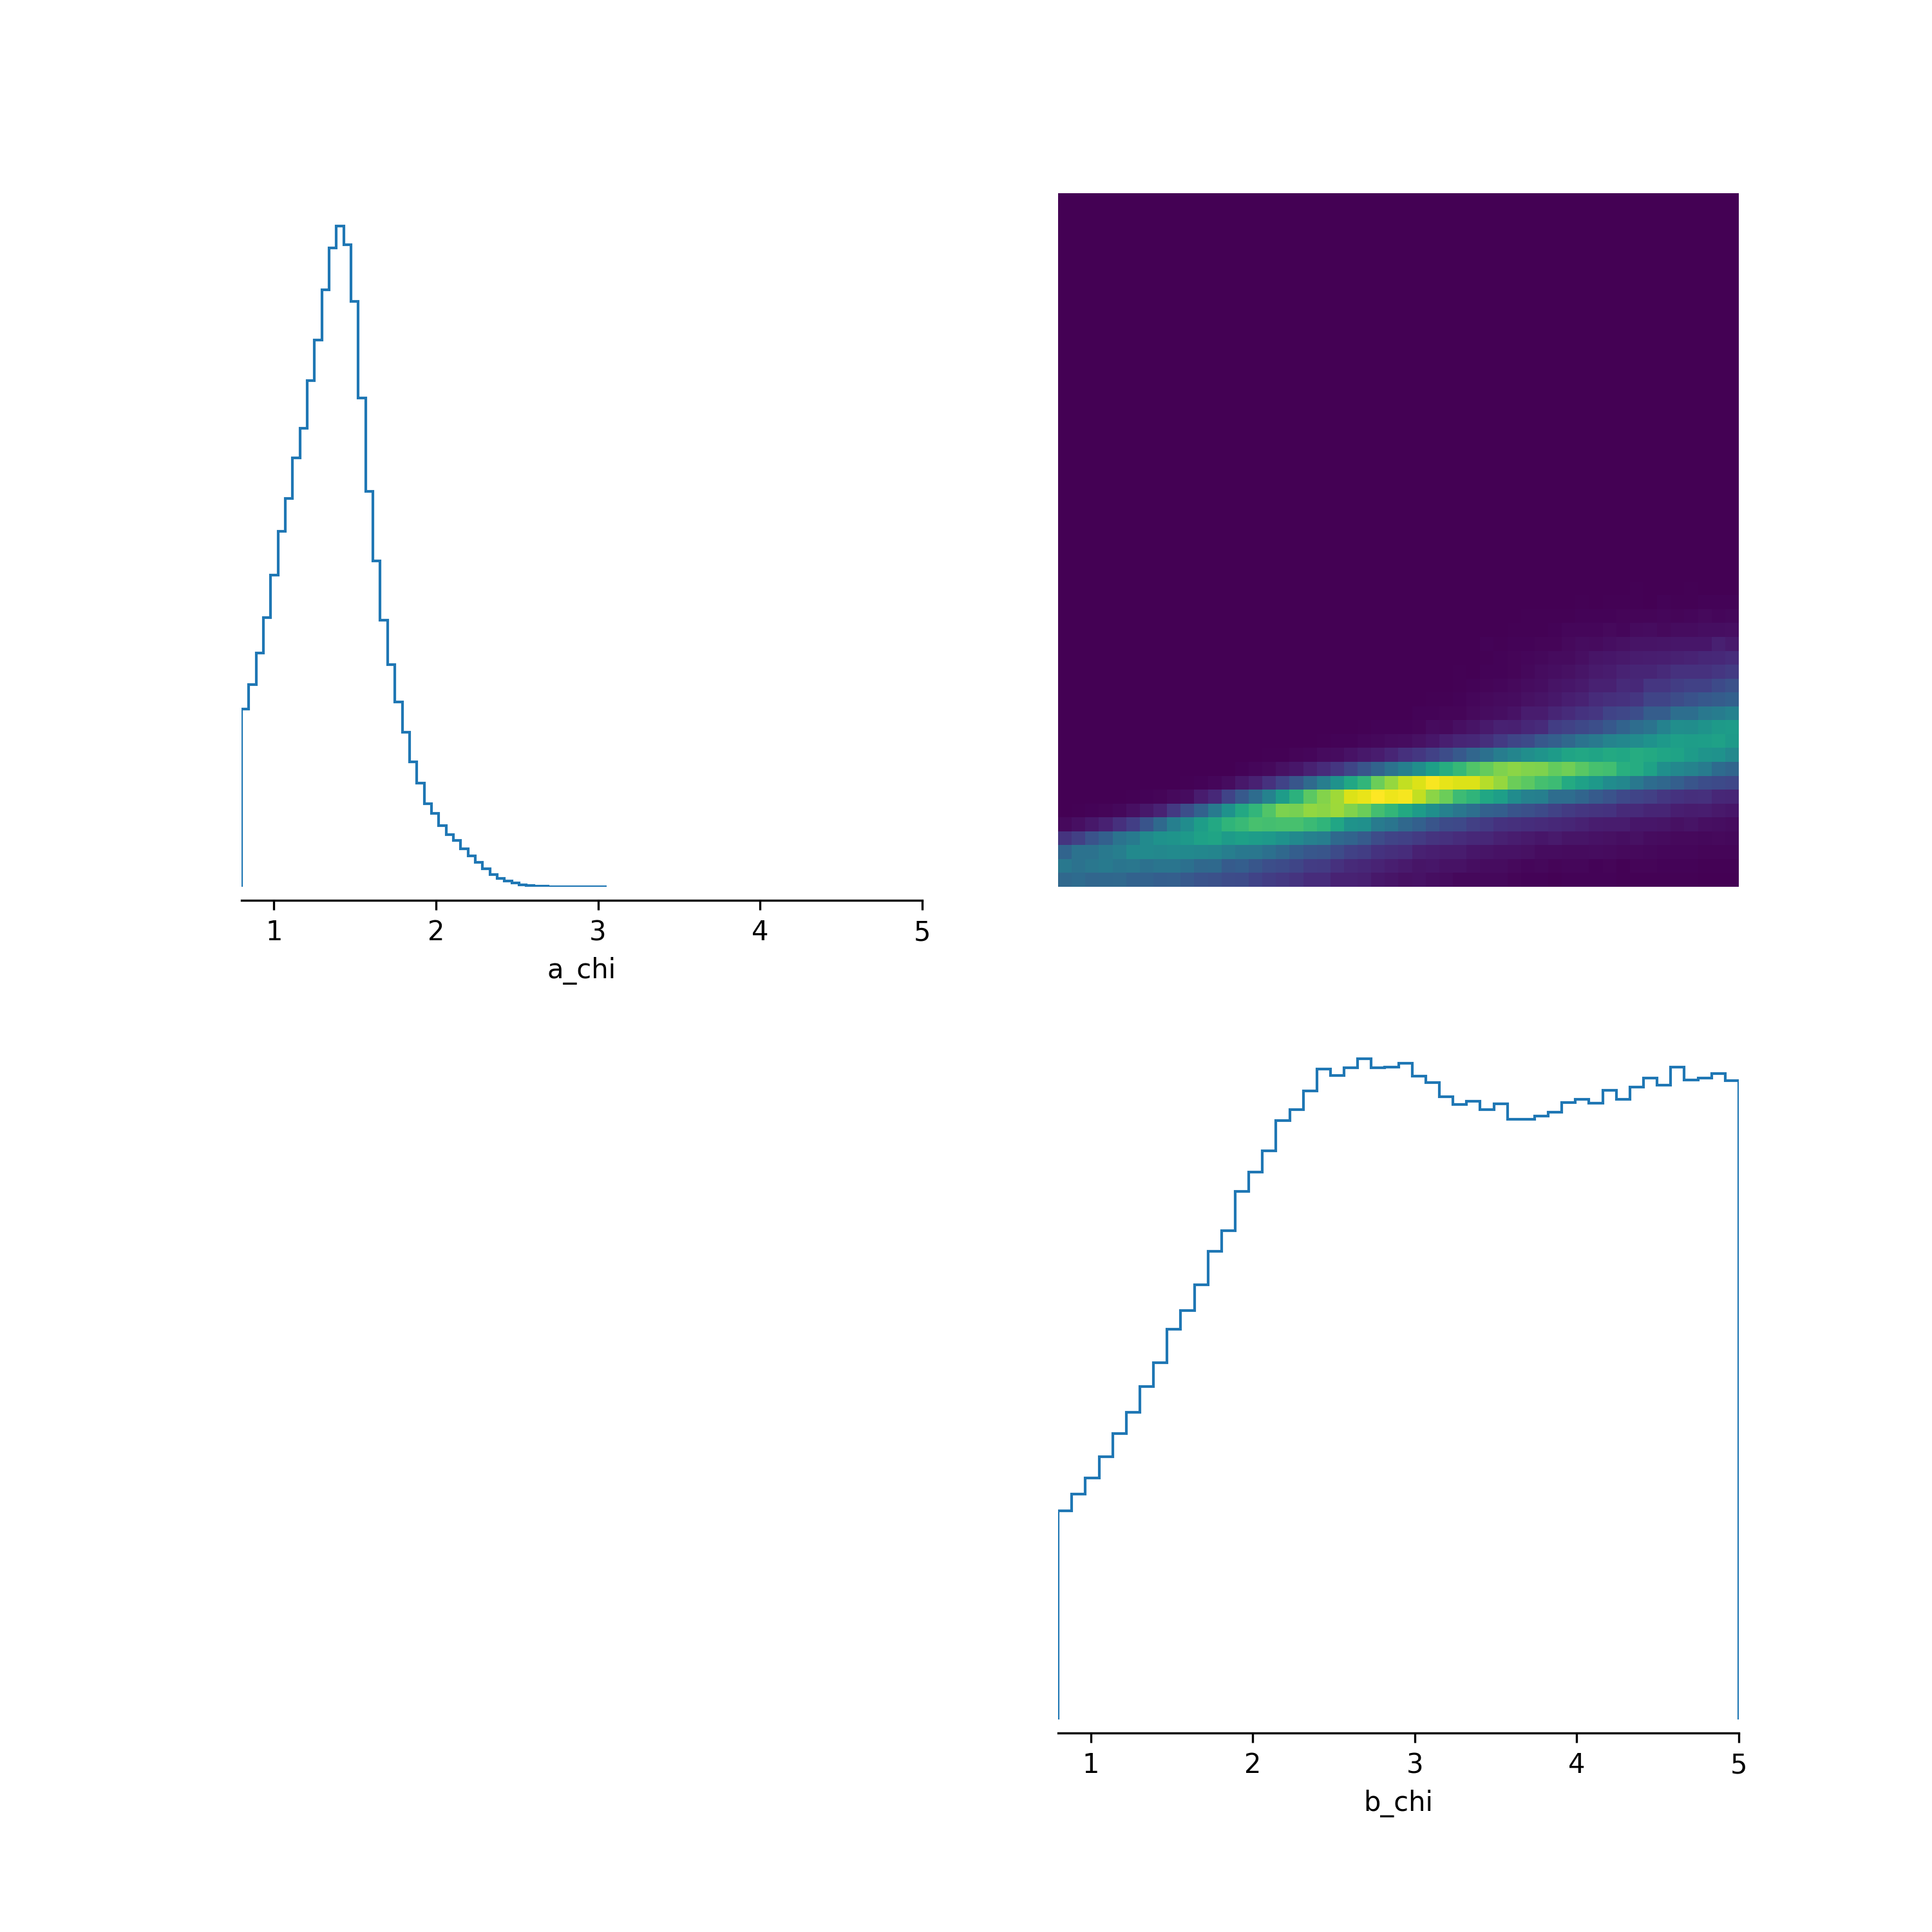
\includegraphics[width=0.7\linewidth]{supplementary_figs/Supp_Figure_1.png}
		\caption{Posterior density for different values of $\alpha_{\chi},\beta_{\chi}$.}
		\label{fig:inference}
	\end{figure}
	
	\begin{figure}[H]
		\centering
		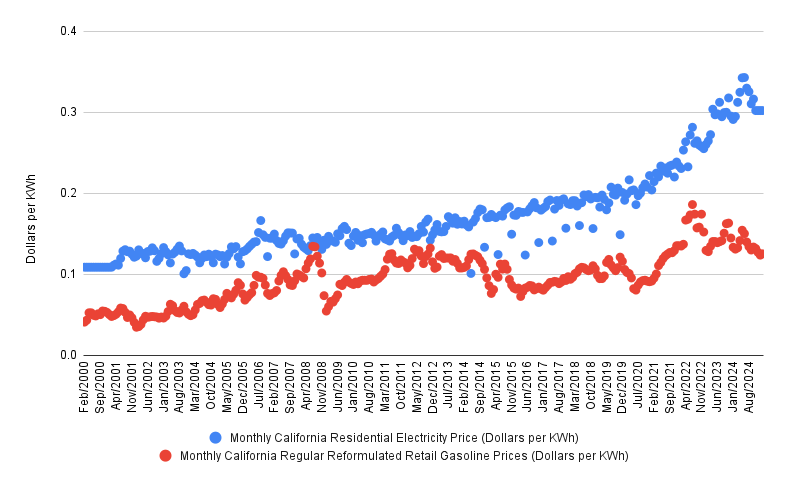
\includegraphics[width=0.85\linewidth]{supplementary_figs/Supp_Figure_2.png}
		\caption{Monthly California Regular Reformulated Retail Gasoline Prices and Residential Electricity Price in Dollars per kilowatt-hour. Source: EIA.}
		\label{fig:Costs_Electricity_Gasoline}
	\end{figure}
	
	\begin{figure}[H]
		\centering
		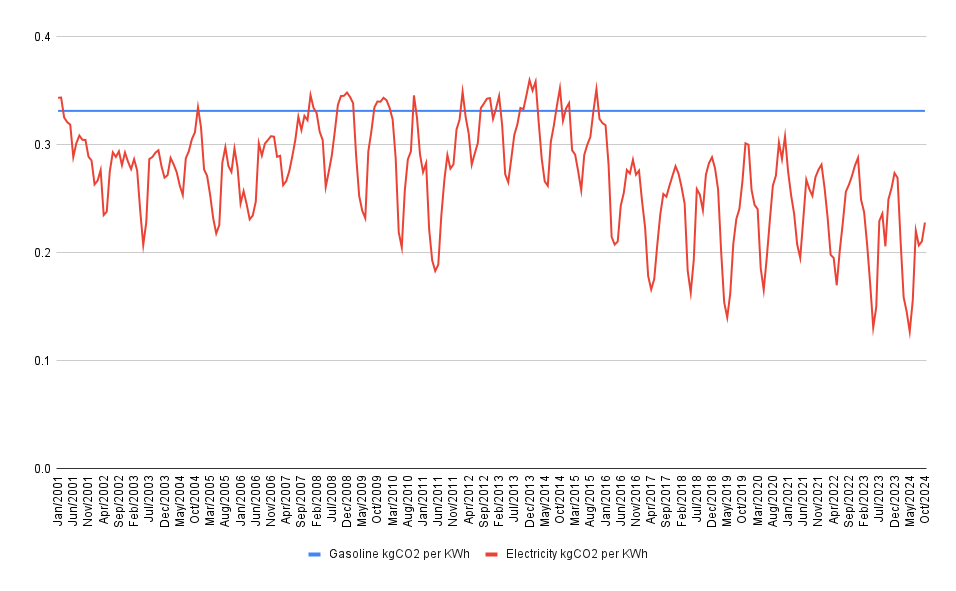
\includegraphics[width=0.85\linewidth]{supplementary_figs/Supp_Figure_3.png}
		\caption{Monthly California Regular Reformulated Retail Gasoline Prices and Residential Electricity Price in Dollars per kilowatt-hour. Source: EIA.}
		\label{fig:Emissions_Electricity_Gasoline}
	\end{figure}
	
	\begin{figure}[H]
		\centering
		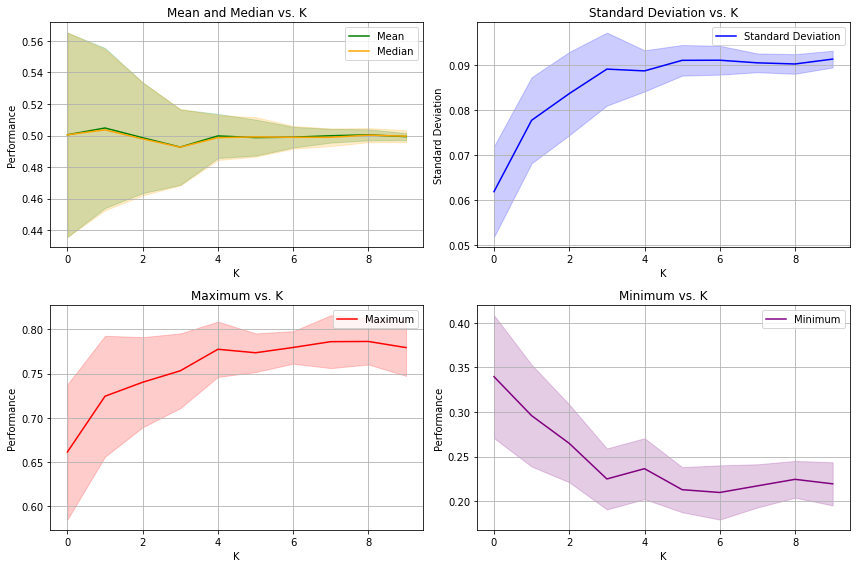
\includegraphics[width=0.85\linewidth]{supplementary_figs/Supp_Figure_4.png}
		\caption{Value distribution in the NK model for different values of K}
		\label{fig:NK}
	\end{figure}
	
	%%%%%%%%%%%%%%%%%%%%%%%%%%%%%%%%%%%%%%%%%%%%%%%%%%%%%%%%%%%%%%%%%%%%%%%%%%%%%%%%%%%%%%%%%%%%%%%%%%%%%%%%%%%%%%%%%%%%

    \begin{figure}[H]
		\centering
		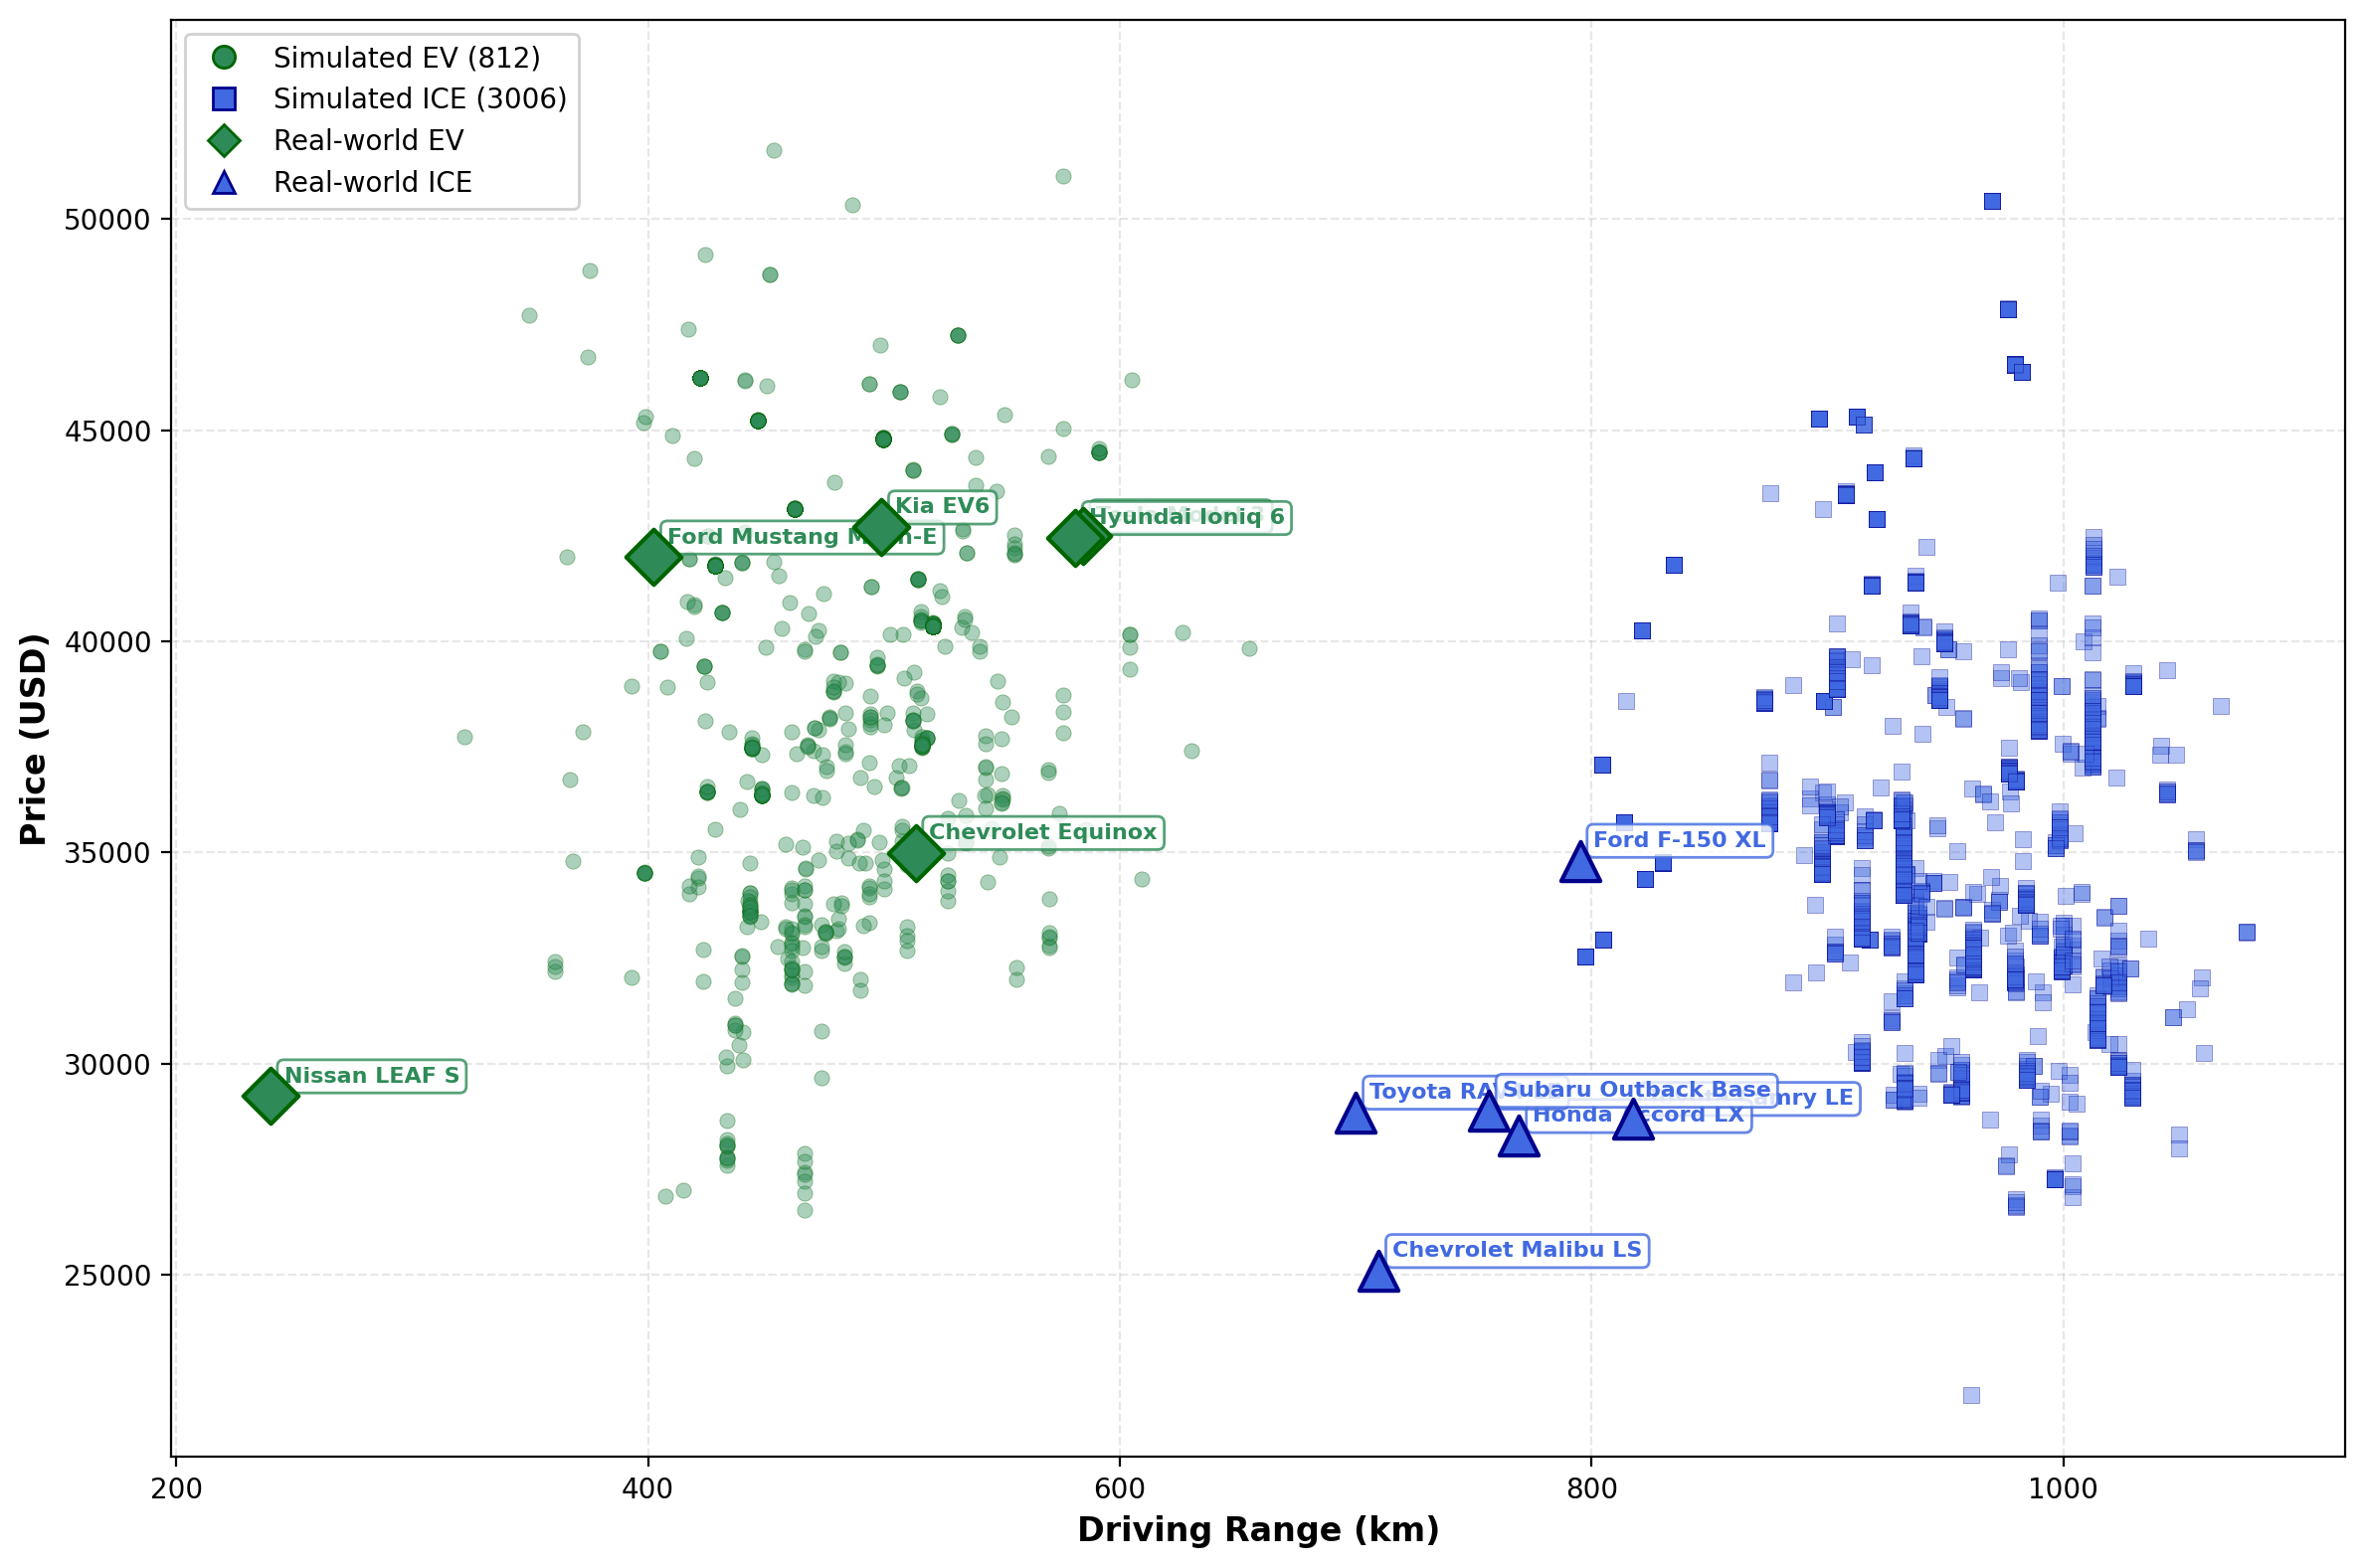
\includegraphics[width=0.85\linewidth]{supplementary_figs/Supp_Figure_5.png}
		\caption{Comparing simulated ICE and EV after calibration period with real-world cars.}
		\label{fig:calibration_cars}
	\end{figure}
    
	\begin{figure}[H]
		\centering
		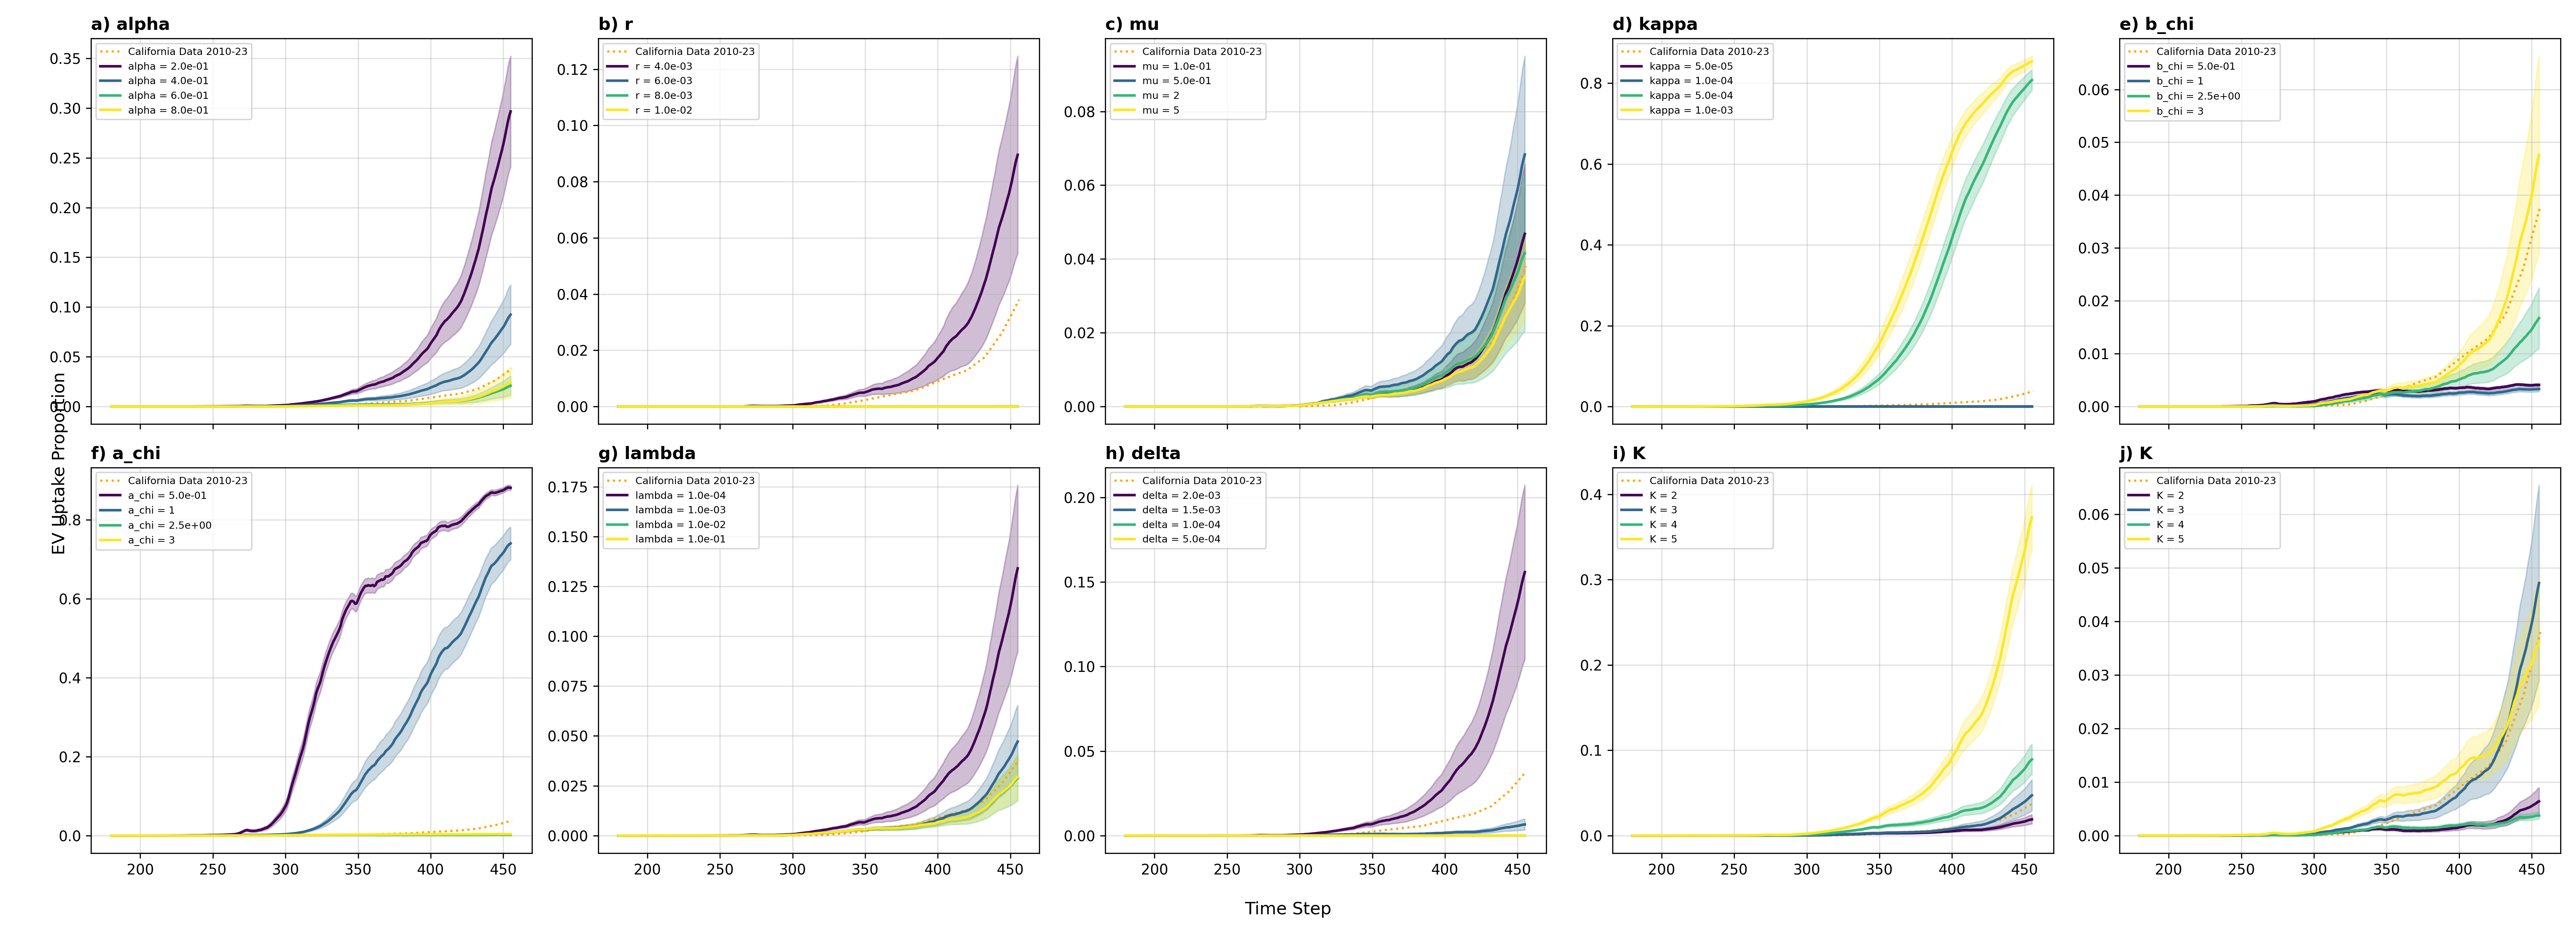
\includegraphics[width=0.9\linewidth]{supplementary_figs/Supp_Figure_6.png}
			\caption{EV uptake proportion for local variation of key parameters.}
			\label{fig:sensitivity}
	\end{figure}
    
	\begin{figure}[H]
		\centering
		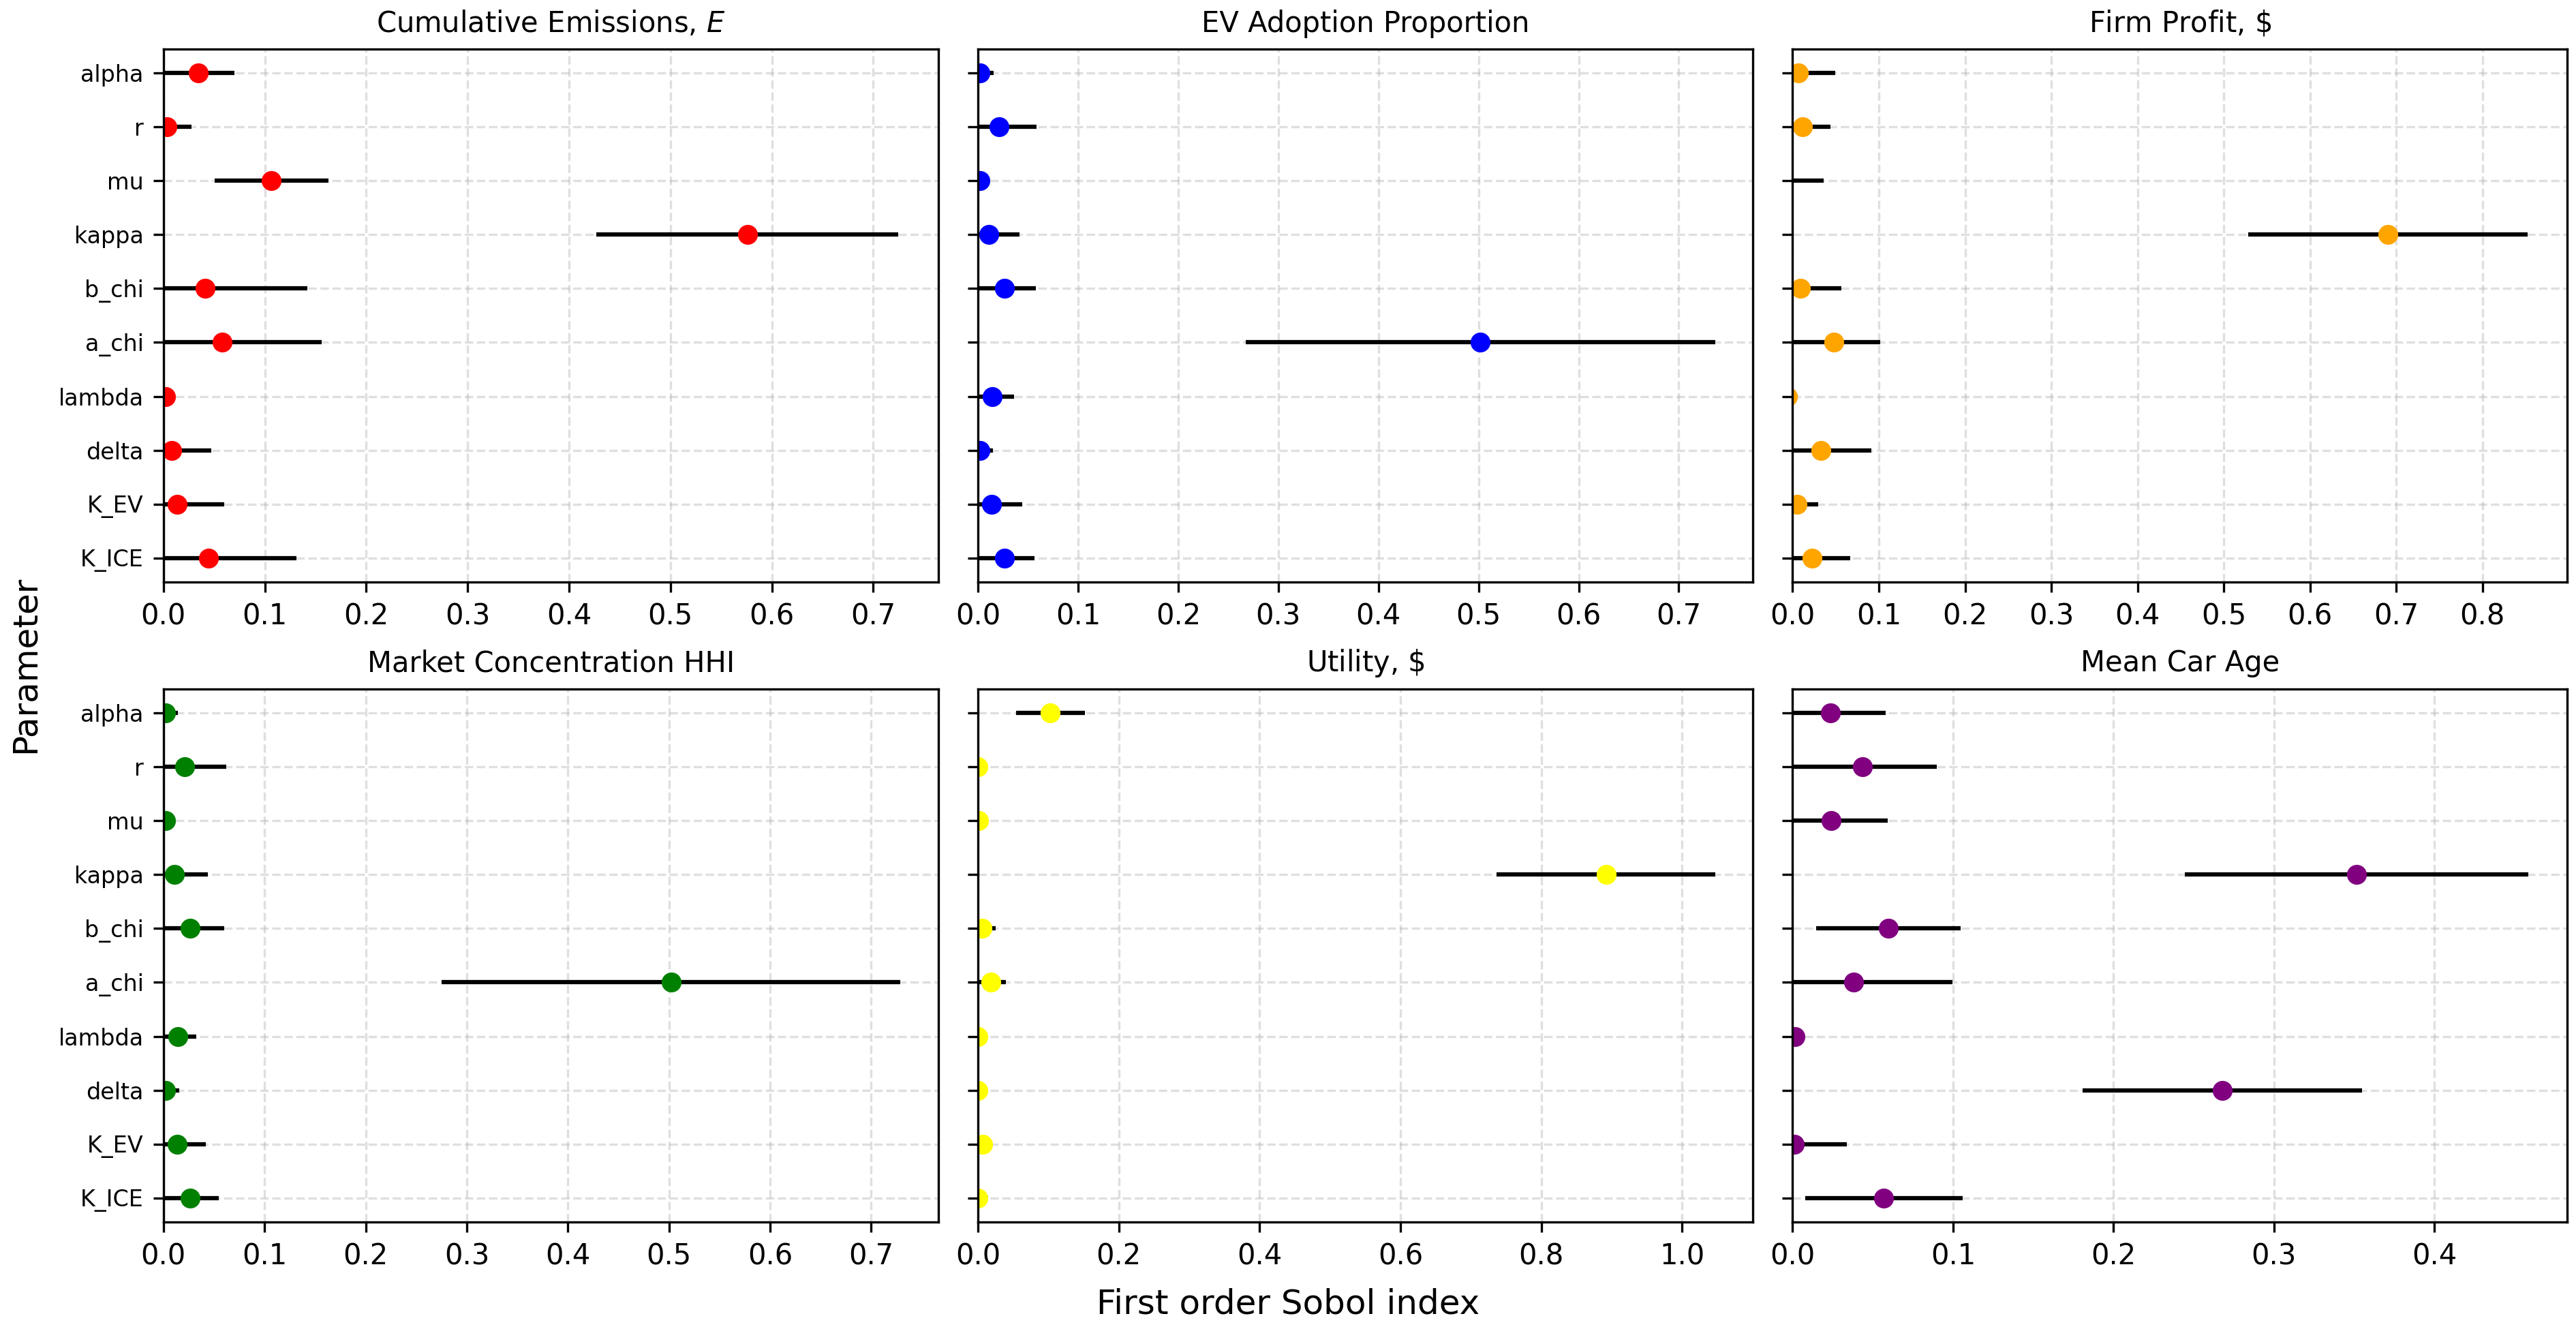
\includegraphics[width=0.9\linewidth]{supplementary_figs/Supp_Figure_7.png}
		\caption{Sobol sensitivity using first order index.}
		\label{fig:sobol_first}
	\end{figure}
	
	\begin{figure}[H]
		\centering
		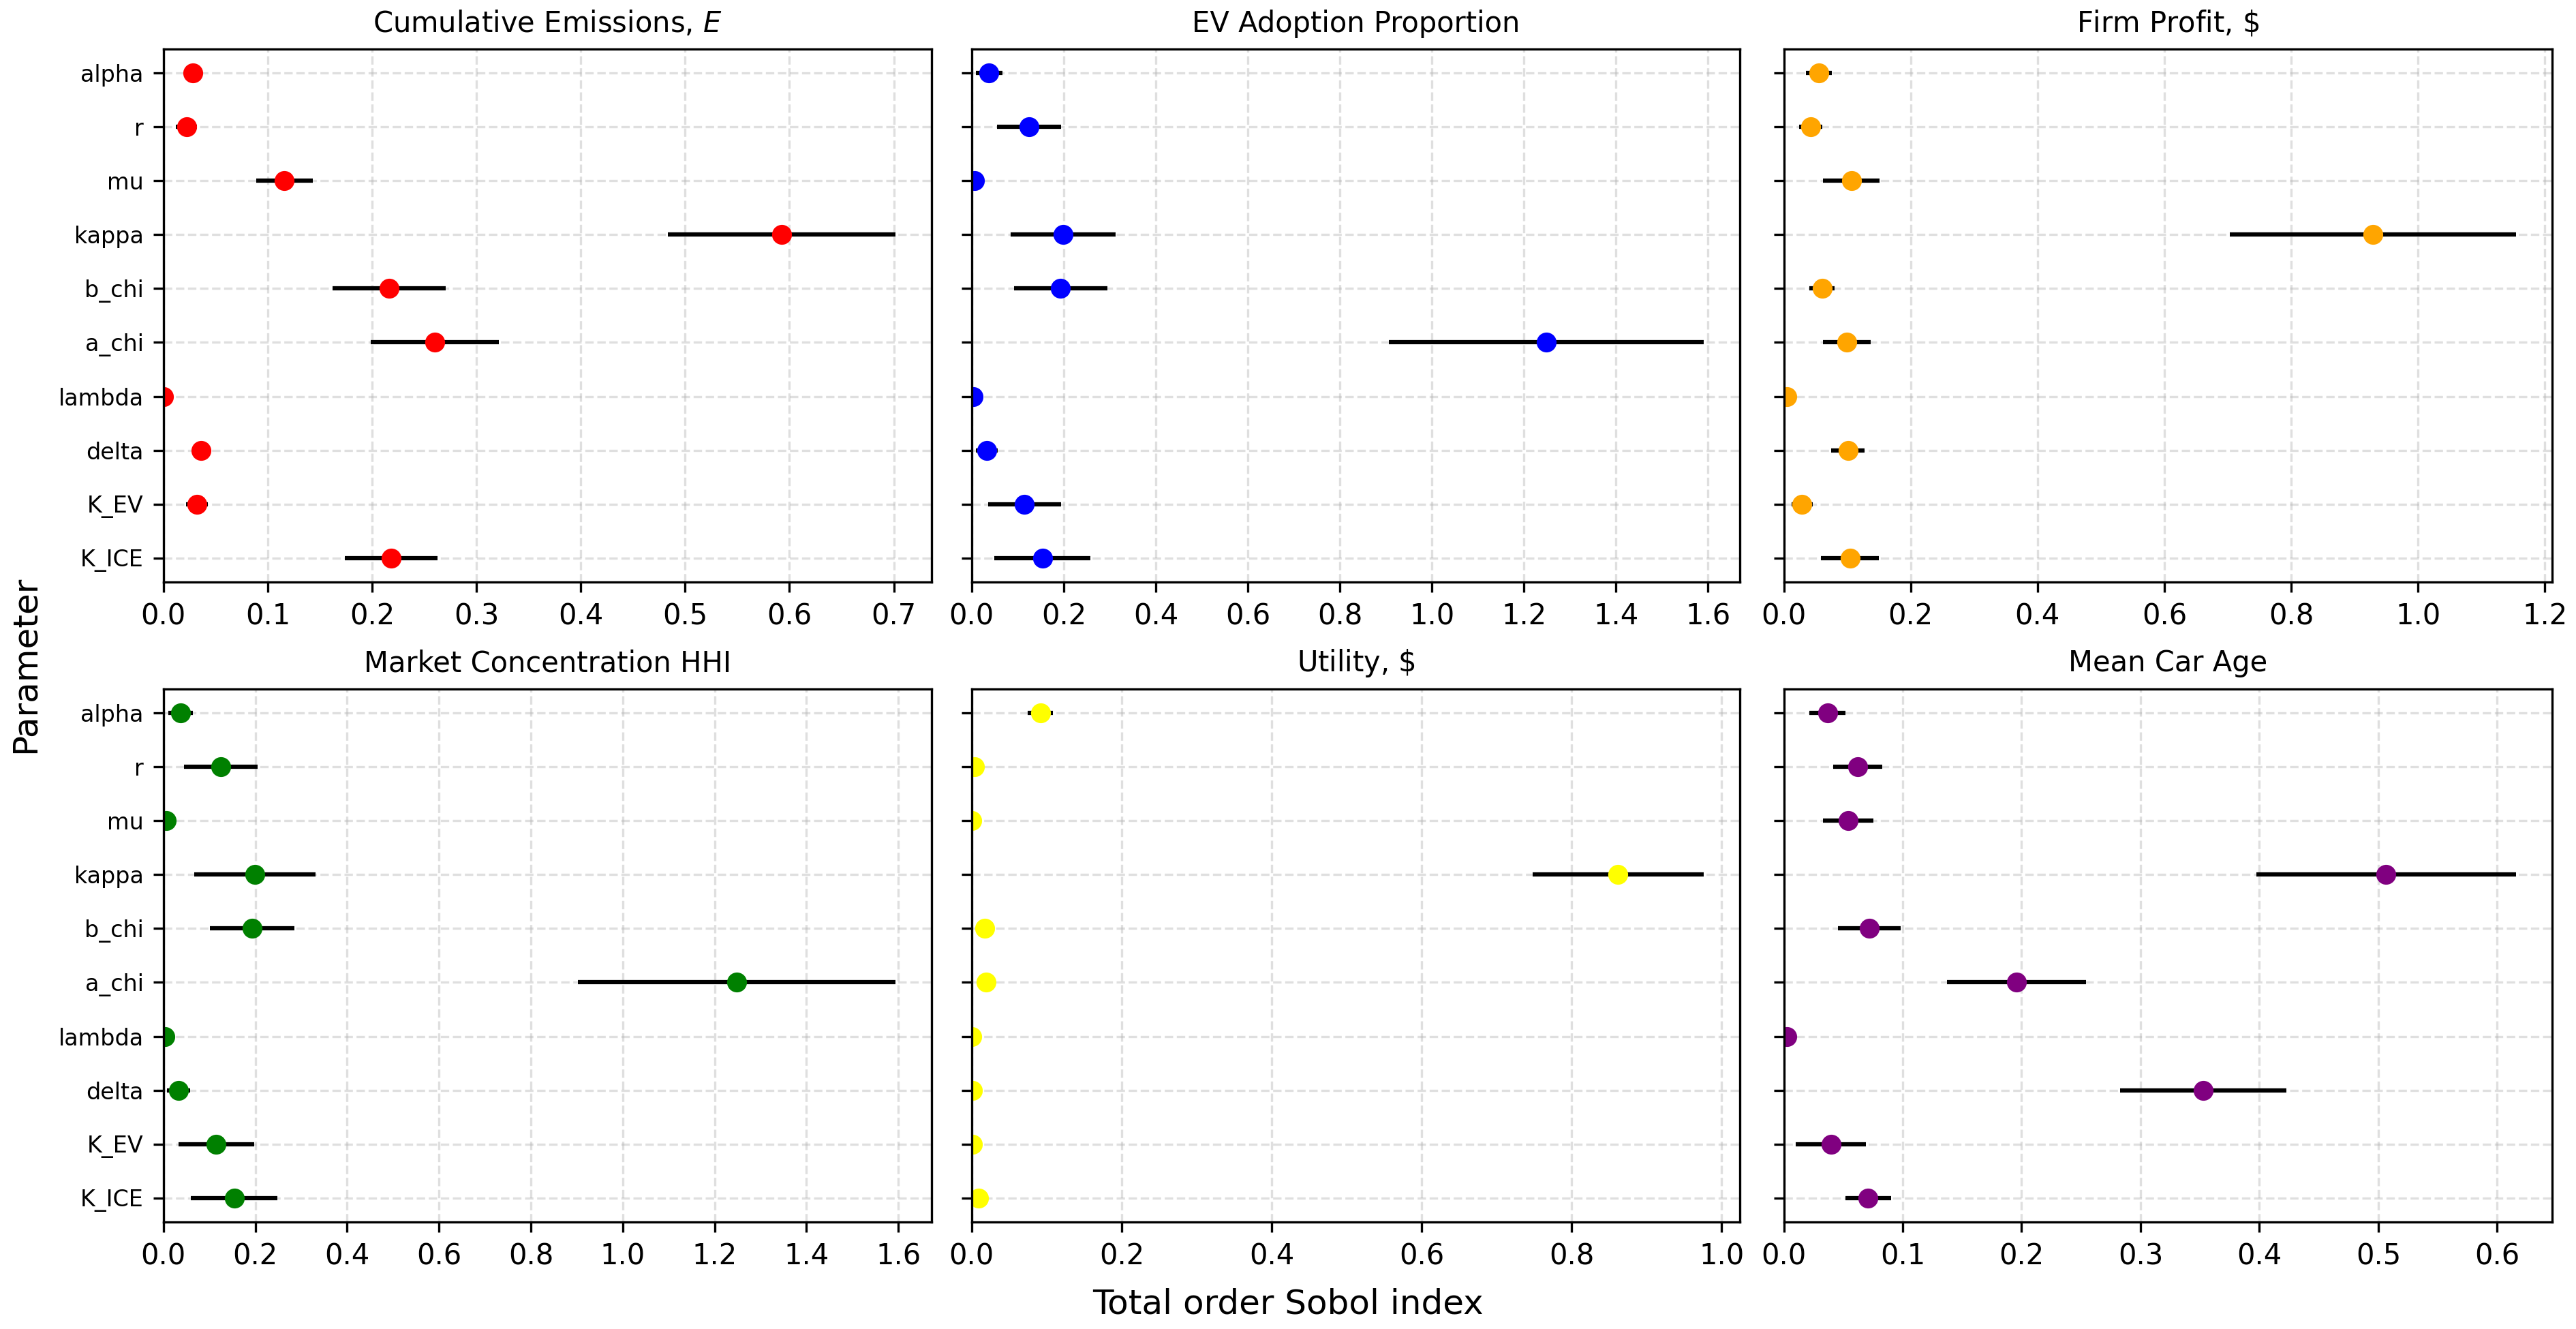
\includegraphics[width=0.9\linewidth]{supplementary_figs/Supp_Figure_8.png}
		\caption{Sobol sensitivity using total order index.}
		\label{fig:sobol_total}
	\end{figure}

	\begin{figure}[H]
		\centering
		\includegraphics[width=0.8\linewidth]{pics/BAU_sen.png}
		\caption{BAU sensitivity in EV uptake (top panels) and Monthly emissions flow (bottom panels) to changes in emissions intensity of electricity and electricity price.}
		\label{fig:BAU_sen_elec}
	\end{figure}

    \begin{figure}[H]
		\centering
		\includegraphics[width=0.8\linewidth]{pics/elasticity_comparison.png}
		\caption{BAU elasticity in EV uptake (top panels) and Monthly emissions flow (bottom panels) to changes in emissions intensity of electricity and electricity price.}
		\label{fig:BAU_sen_elec_elas}
	\end{figure}

    \begin{figure}[H]
		\centering
		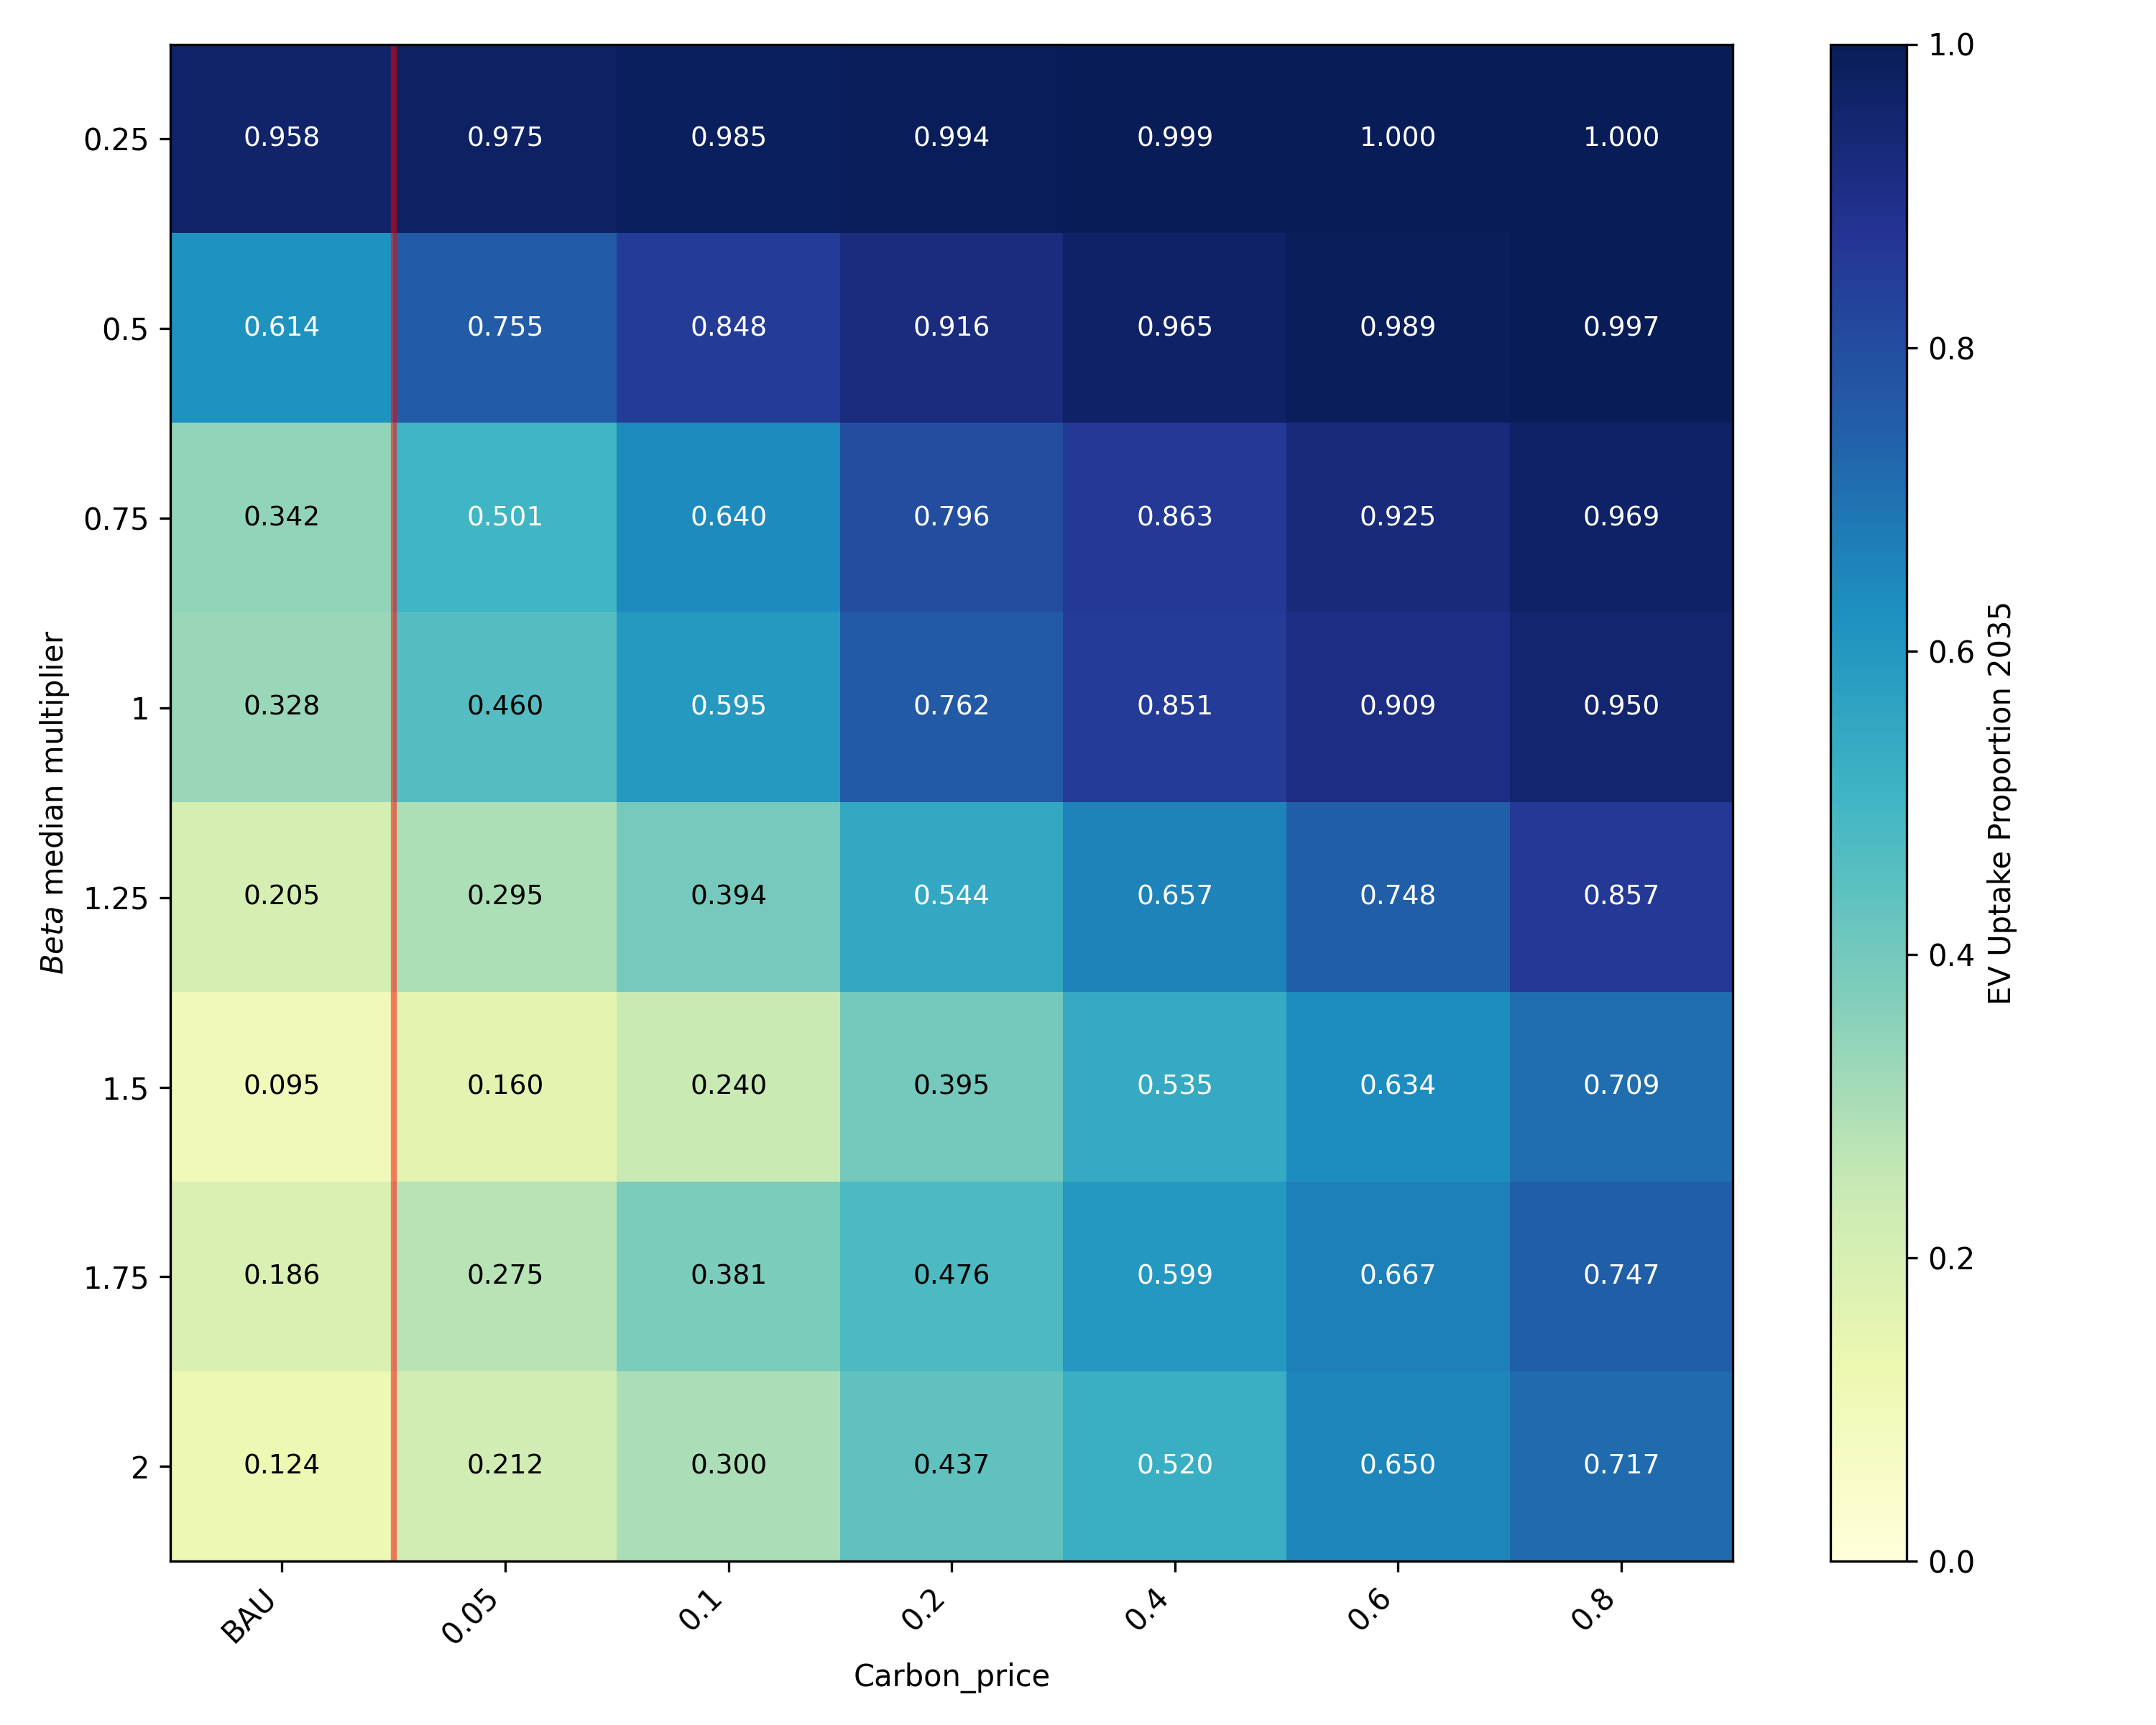
\includegraphics[width=0.8\linewidth]{supplementary_figs/Supp_Figure_11.png}
		\caption{EV uptake for combinations of multiplier of median willingness-to-pay for quality, a proxy of average consumer price sensitivity and carbon price.}
		\label{fig:WTP_sensitivity_carbon_price}
	\end{figure}

    \begin{figure}[H]
		\centering
		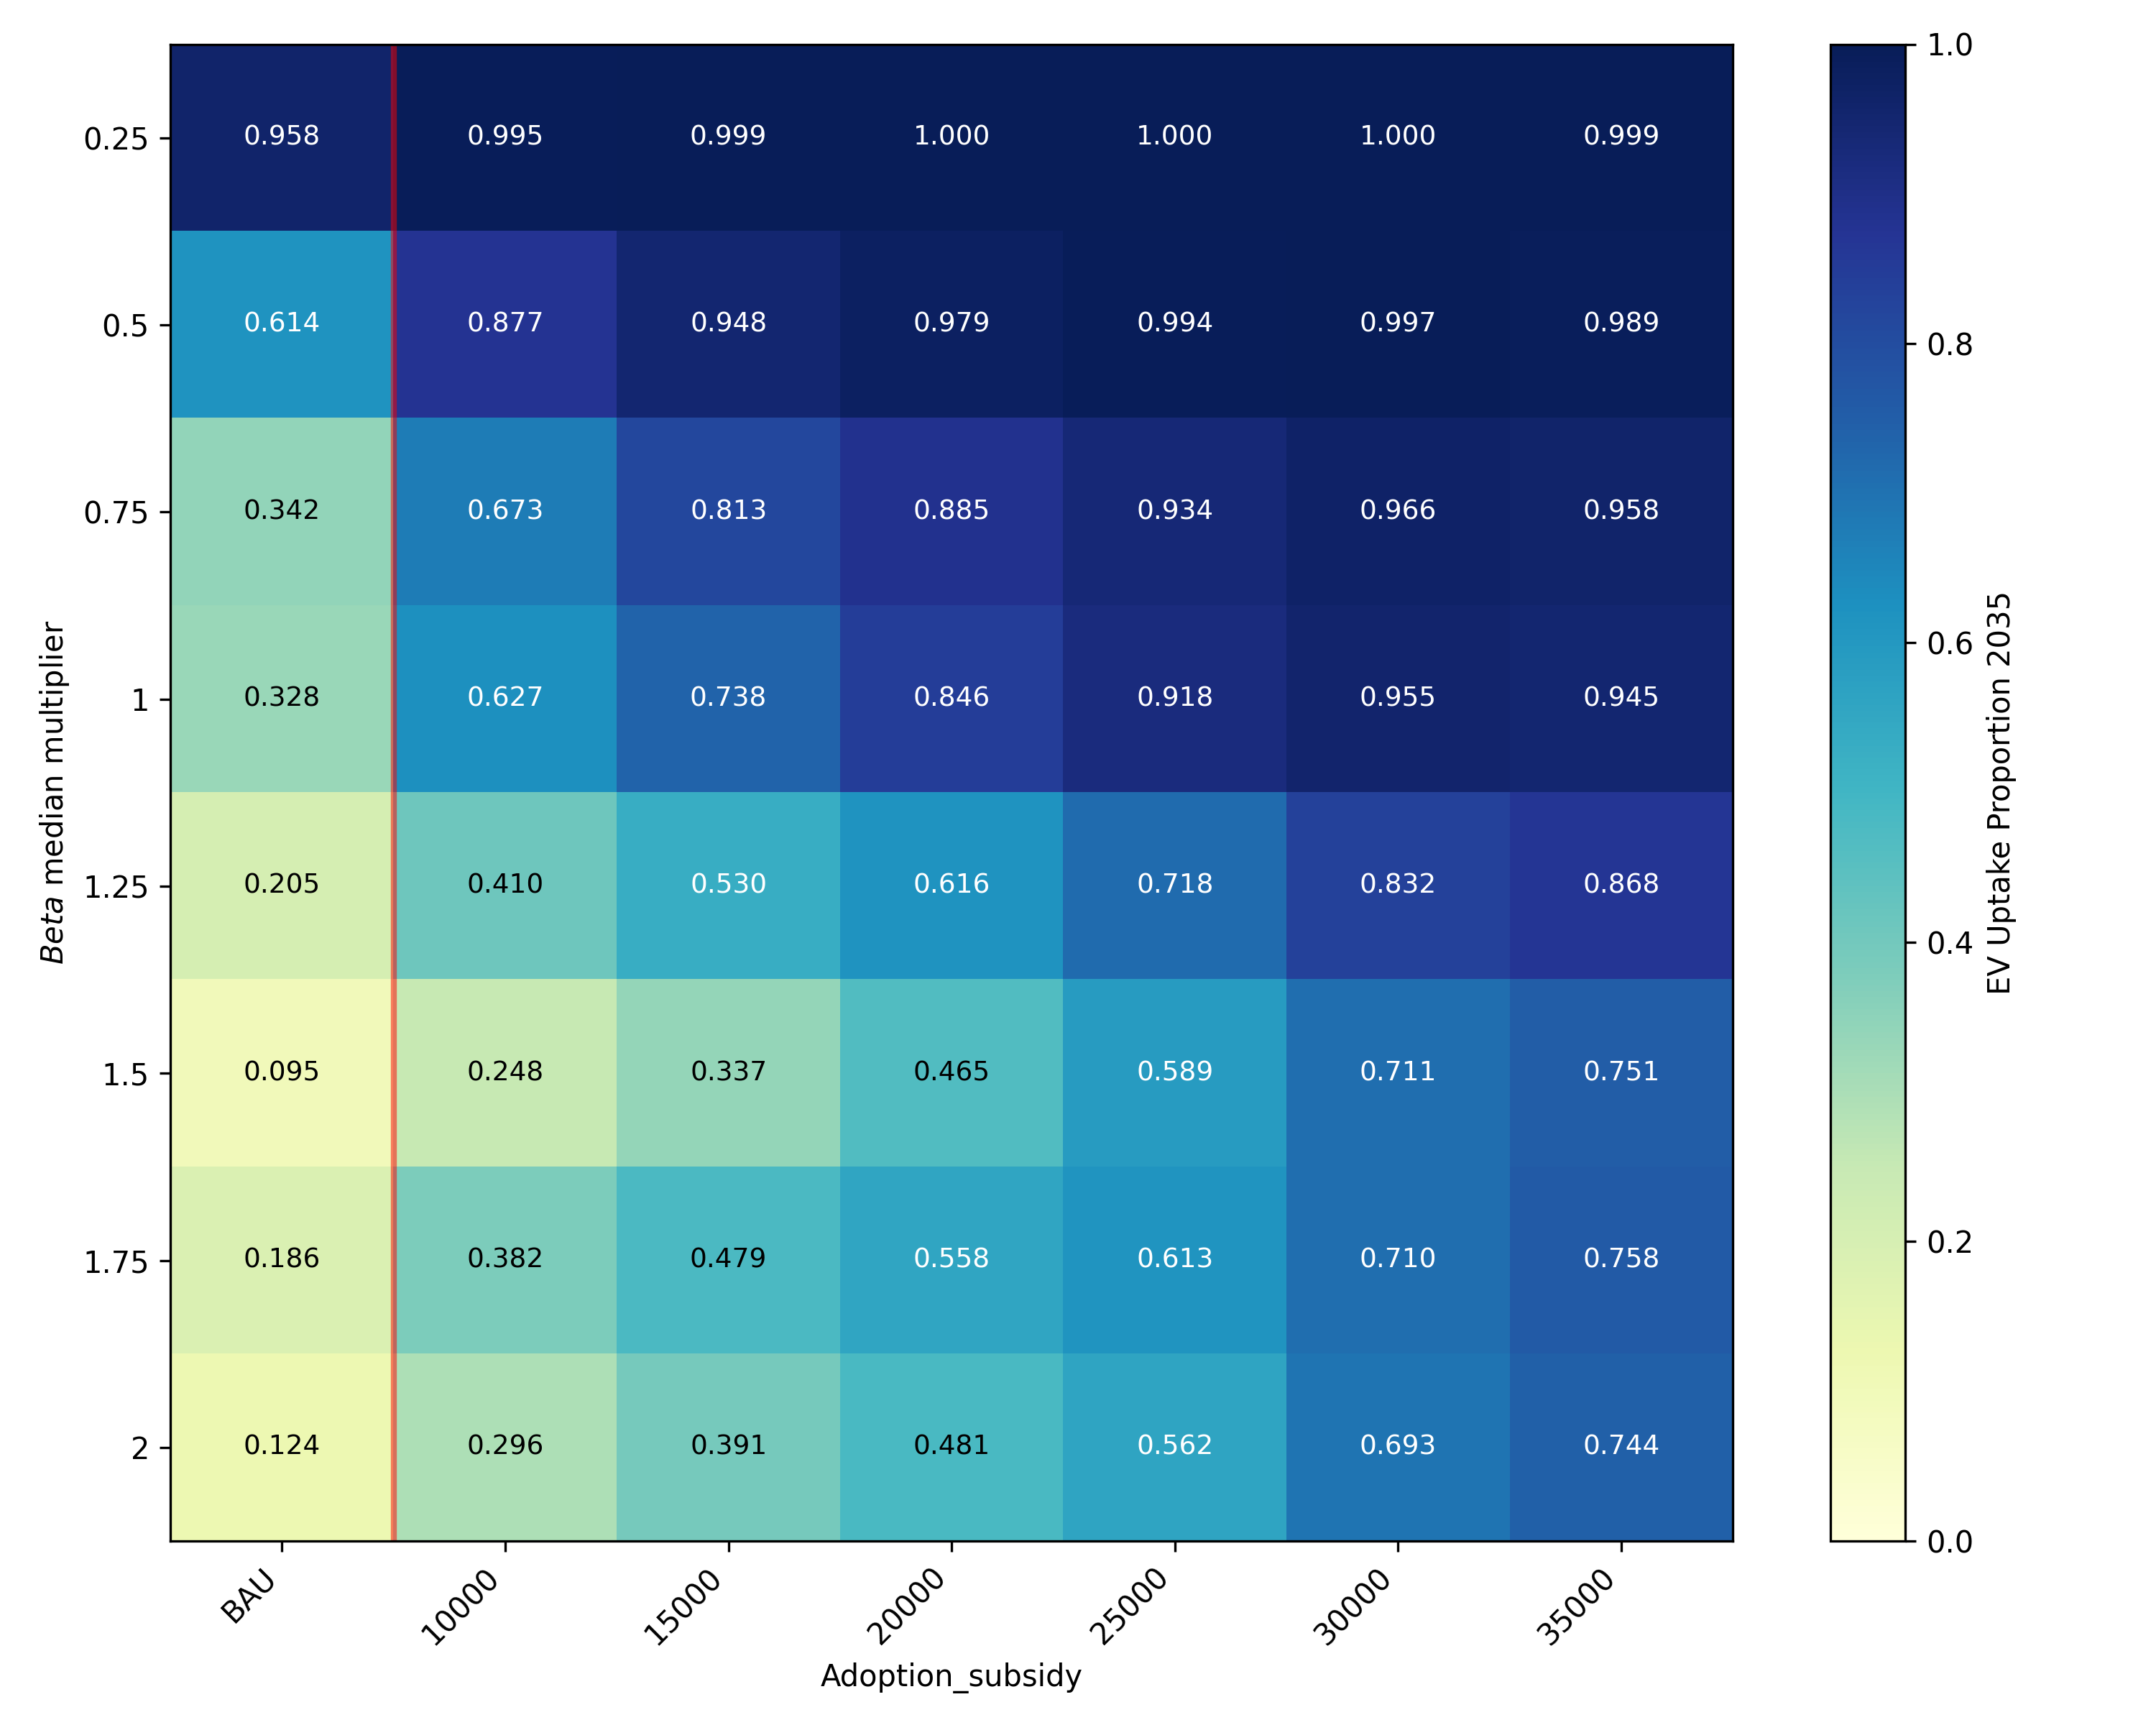
\includegraphics[width=0.8\linewidth]{supplementary_figs/Supp_Figure_12.png}
		\caption{EV uptake for combinations of multiplier of median willingness-to-pay for quality, a proxy of average consumer price sensitivity and new car rebate.}
		\label{fig:WTP_sensitivity_adoption_subsidy}
	\end{figure}
    
    \begin{figure}[H]
		\centering
		\includegraphics[width=0.8\linewidth]{pics/a_chi_carbon_price.png}
		\caption{EV uptake for combinations of thresholds to EV adoption, $a_{\chi}$ and carbon price.}
		\label{fig:a_chi_carbon_price}
	\end{figure}

    \begin{figure}[H]
		\centering
		\includegraphics[width=0.8\linewidth]{pics/a_chi_adoption_subsidy.png}
		\caption{EV uptake for combinations of thresholds to EV adoption, $a_{\chi}$ and new car rebate.}
		\label{fig:a_chi_adoption_subsidy}
	\end{figure}
	
	\printbibliography
	%\bibliography{bib.bib}
	\end{document}
